\documentclass[11pt,a4paper]{article}

% Typography and encoding
\usepackage[utf8]{inputenc}
\usepackage[T1]{fontenc}
\usepackage{lmodern}

% Page geometry
\usepackage[margin=2.2cm]{geometry}

% Mathematics
\usepackage{amsmath, amssymb, amsfonts, mathtools}

% Lists and tables
\usepackage[shortlabels]{enumitem}
\usepackage{booktabs}
\usepackage{array}

% Units and graphics
\usepackage{siunitx}
\usepackage{graphicx}
\usepackage[american]{circuitikz}
\usepackage{tikz}
\usetikzlibrary{arrows.meta, positioning, calc}

% Colors and hyperlinks
\usepackage{xcolor}
\usepackage[
    colorlinks=true,
    linkcolor=blue!70!black,
    citecolor=blue!70!black,
    urlcolor=blue!70!black,
    pdfauthor={Bertrand Cornélusse, Geoffrey},
    pdftitle={ELEC0447 - Analysis of Electrical Power and Energy Systems: Exercise Manual}
]{hyperref}

% Document Header
\title{
    \textbf{ELEC0447 -- Analysis of Electrical Power and Energy Systems} \\
    \vspace{0.4em}
    \Large Practical Sessions (TP 1 to 6) -- Exercise Manual \\
    \large Problem Statements and Step-by-Step Solutions
}
\author{
    \textbf{Prof. Bertrand Cornélusse} \\
    \textit{Based on exercise formulations and solution notes by Geoffrey and the teaching team} \\
    Department of Electrical Engineering and Computer Science (Montefiore Institute) \\
    University of Liège
}
\date{Academic Year 2026--2027}

\begin{document}

\maketitle

\begin{abstract}
This document gathers the complete problem statements and rigorous, step-by-step solutions to the practical exercise sessions (TP 1 through TP 6) for the course \textbf{ELEC0447: Analysis of Electrical Power and Energy Systems}. It covers: phasor-domain circuit analysis and power factor correction (TP 1); three-phase circuits, power transfer between AC systems, radial voltage profiles, and the per-unit system (TP 2); transmission line Surge Impedance Loading (SIL), Joule losses, and distributed Telegrapher's wave equations (TP 3); ideal and non-ideal transformer modeling with and without per-unit formalism (TP 4); synchronous generator steady-state/transient reactances, power-angle characteristics, and excitation control (TP 5); and voltage instability, analytical derivation of the $P$-$V$ nose curve, maximum transmissible active power $P_{\text{max}}$, critical voltage, and reactive power compensation effects (TP 6).
\end{abstract}

\vspace{1.5em}
\tableofcontents
\newpage

% Include practical sessions
\section{Practical Session 1: Phasor-Domain Analysis}

\subsection{Exercises}
\begin{enumerate}
    \item \textbf{Phasor Representation of Sinusoidal Voltages}\footnote{Exercises 2.1, 2.2, 2.5 and 2.9 from Ned Mohan's book \textit{"Electric power systems, a first course"}.}
    
    Express the following voltages as phasors:
    \begin{enumerate}
        \item $v_1(t) = \sqrt{2} \times 100 \cos(\omega t - 30^\circ)\ \text{V}$
        \item $v_2(t) = \sqrt{2} \times 100 \cos(\omega t + 30^\circ)\ \text{V}$
    \end{enumerate}

    \item \textbf{Series $R$-$L$-$C$ Circuit}
    
    The series $R$-$L$-$C$ circuit shown in Figure~\ref{fig:tp1_rlc} is in sinusoidal steady state at a frequency of $f = 60\ \text{Hz}$. The parameters are:
    \[
    V = 120\ \text{V},\quad R = 1.5\ \Omega,\quad L = 20\ \text{mH},\quad C = 100\ \mu\text{F}.
    \]
    Calculate the current $i(t)$ in this circuit by using phasor-domain analysis.

    \begin{figure}[htbp]
        \centering
        \begin{circuitikz}[american, scale=1.1]
            \draw (0,0) to[sV, v_>=$v(t){=}\sqrt{2}V\cos(\omega t)$] (0,3)
                  to[short, i=$i(t)$] (2,3)
                  to[L, l=$L$] (3.5,3)
                  to[R, l=$R$] (3.5,1.5)
                  to[C, l=$C$] (3.5,0)
                  -- (0,0);
        \end{circuitikz}
        \caption{Series $R$-$L$-$C$ circuit.}
        \label{fig:tp1_rlc}
    \end{figure}

    \item \textbf{Series-Parallel $R$-$L$-$C$ Circuit and Reactive Power Conservation}
    
    To the circuit of Figure~\ref{fig:tp1_ex4}, if a voltage of $100\angle 0^\circ\ \text{V}$ is applied, calculate the active power $P$, the reactive power $Q$, and the power factor $\cos\phi$. Show that:
    \[
    Q = \sum_k I_k^2 X_k
    \]

    \begin{figure}[htbp]
        \centering
        \begin{circuitikz}[american, scale=1.1]
            \draw (0,0) to[sV, v_>=$\bar{V}{=}100\angle 0^\circ\ \text{V}$] (0,2.5)
                  to[L, l=$j0.1\ \Omega$, i=$\bar{I}_L$] (3,2.5)
                  -- (4.5,2.5);
            \draw (3,2.5) to[C, l=$-j5\ \Omega$, i=$\bar{I}_C$] (3,0);
            \draw (4.5,2.5) to[R, l=$2\ \Omega$, i=$\bar{I}_R$] (4.5,0);
            \draw (0,0) -- (4.5,0);
        \end{circuitikz}
        \caption{Series-parallel circuit for Exercise 3.}
        \label{fig:tp1_ex4}
    \end{figure}

    \item \textbf{Power Factor Correction}
    
    In the circuit of Figure~\ref{fig:tp1_pfc}, the complex power drawn by the load impedance is:
    \[
    S_L = P_L + j Q_L = (1858.4 + j1031.3)\ \text{VA}.
    \]
    Calculate the capacitive reactance $X_C$ connected in parallel necessary to make the overall power factor equal to $0.9$ (leading), assuming the applied voltage has an RMS value of $V = 120\ \text{V}$ at $f = 60\ \text{Hz}$. Determine the required capacitance $C$.

    \begin{figure}[htbp]
        \centering
        \begin{circuitikz}[american, scale=1.1]
            \draw (0,0) to[sV, v_>=$\bar{V}_1$] (0,3)
                  to[short, i=$P{=}P_L$] (2.5,3)
                  -- (4.5,3);
            \draw (2.5,3) to[C, l=$-j Q_C$, i>^=$Q_C$] (2.5,0);
            \draw (4.5,3) to[generic, l={$P_L + j Q_L$}, i>^={$P_L + j Q_L$}] (4.5,0);
            \draw (0,0) -- (4.5,0);
        \end{circuitikz}
        \caption{Power factor correction circuit.}
        \label{fig:tp1_pfc}
    \end{figure}
\end{enumerate}

\newpage
\subsection{Solutions}

\subsubsection*{Solution to Exercise 1: Phasor Representation}
Using the cosine reference with RMS value as phasor magnitude:
\begin{align*}
    v(t) = \sqrt{2} V_{\text{RMS}} \cos(\omega t + \theta) \iff \bar{V} = V_{\text{RMS}} e^{j\theta} = V_{\text{RMS}} \angle \theta
\end{align*}

\begin{enumerate}[(a)]
    \item For $v_1(t) = \sqrt{2} \times 100 \cos(\omega t - 30^\circ)\ \text{V}$:
    \begin{equation}
        \boxed{\bar{V}_1 = V_{\text{RMS}} e^{j\theta} = \frac{V_m}{\sqrt{2}} e^{-j 30^\circ} = 100\ \text{V} \angle -30^\circ}
    \end{equation}

    \item For $v_2(t) = \sqrt{2} \times 100 \cos(\omega t + 30^\circ)\ \text{V}$:
    \begin{equation}
        \boxed{\bar{V}_2 = V_{\text{RMS}} e^{j\theta} = \frac{V_m}{\sqrt{2}} e^{+j 30^\circ} = 100\ \text{V} \angle +30^\circ}
    \end{equation}
\end{enumerate}

\subsubsection*{Solution to Exercise 2: Series $R$-$L$-$C$ Circuit}
\paragraph{Data:}
\begin{itemize}
    \item Voltage: $\bar{V} = 120\ \text{V}\angle 0^\circ$
    \item Resistance: $R = 1.5\ \Omega$
    \item Inductance: $L = 20\ \text{mH} = 20 \times 10^{-3}\ \text{H}$
    \item Capacitance: $C = 100\ \mu\text{F} = 100 \times 10^{-6}\ \text{F}$
    \item Frequency: $f = 60\ \text{Hz} \implies \omega = 2\pi f = 2\pi \times 60 = 376.99\ \text{rad/s}$
\end{itemize}

\paragraph{Impedance $Z$:}
The total impedance of the series circuit is:
\begin{align}
    Z &= R + j\omega L + \frac{1}{j\omega C} = R + j\left(\omega L - \frac{1}{\omega C}\right) \nonumber\\
      &= 1.5 + j\left(376.99 \times 20 \times 10^{-3} - \frac{1}{376.99 \times 100 \times 10^{-6}}\right) \nonumber\\
      &= 1.5 + j(7.5398 - 26.5258) = 1.5 - j18.986\ \Omega \nonumber\\
      &= 19.049\ \Omega \angle -85.48^\circ\quad (-1.492\ \text{rad})
\end{align}

\paragraph{Current Phasor $\bar{I}$:}
By Ohm's law:
\begin{equation}
    \bar{I} = \frac{\bar{V}}{Z} = \frac{120\angle 0^\circ}{19.049\angle -85.48^\circ} = 6.30\ \text{A} \angle +85.48^\circ\quad (+1.492\ \text{rad})
\end{equation}

\paragraph{Time-Domain Current $i(t)$:}
Converting back from the RMS phasor to the time domain:
\begin{equation}
    \boxed{i(t) = 6.30\sqrt{2} \cos(376.99 t + 1.492)\ \text{A} = 8.91 \cos(376.99 t + 85.5^\circ)\ \text{A}}
\end{equation}

\subsubsection*{Solution to Exercise 3: Series-Parallel Circuit and Power Conservation}
\paragraph{Data:}
\begin{itemize}
    \item Applied voltage: $\bar{V} = 100\ \text{V} \angle 0^\circ$
    \item Inductor impedance: $Z_L = j0.1\ \Omega$
    \item Capacitor impedance: $Z_C = -j5\ \Omega$
    \item Resistor impedance: $R = 2\ \Omega$
\end{itemize}

\paragraph{Total Equivalent Impedance $Z$:}
The capacitor and resistor are connected in parallel:
\begin{align}
    Z_p = Z_C \parallel R = \frac{R \cdot Z_C}{R + Z_C} = \frac{2(-j5)}{2 - j5} = \frac{-j10(2 + j5)}{2^2 + (-5)^2} = \frac{50 - j20}{29} = 1.7241 - j0.6897\ \Omega
\end{align}
Adding the series inductor:
\begin{align}
    Z &= Z_L + Z_p = j0.1 + (1.7241 - j0.6897) = 1.7241 - j0.5897\ \Omega \nonumber\\
      &= 1.822\ \Omega \angle -18.88^\circ
\end{align}

\paragraph{Complex Power $S$:}
\begin{align}
    S &= \bar{V} \bar{I}^* = \bar{V} \left(\frac{\bar{V}}{Z}\right)^* = \frac{V^2}{Z^*} = \frac{100^2}{1.822\angle +18.88^\circ} \nonumber\\
      &= 5487.93\ \text{VA} \angle -18.88^\circ
\end{align}
Since $S = P + jQ$:
\begin{align}
    \boxed{P = \text{Re}\{S\} = 5487.93 \cos(-18.88^\circ) = 5192.54\ \text{W}} \\
    \boxed{Q = \text{Im}\{S\} = 5487.93 \sin(-18.88^\circ) = -1775.89\ \text{var}}
\end{align}

\paragraph{Power Factor $\cos\phi$:}
\begin{equation}
    \boxed{\cos\phi = \frac{P}{|S|} = \frac{5192.54}{5487.93} = 0.946\quad (\text{leading})}
\end{equation}
Because $Q < 0$ (and $\phi < 0$), the circuit is capacitive overall: it produces net reactive power, meaning that the current phasor leads the voltage phasor.

\paragraph{Proof that $Q = \sum_k I_k^2 X_k$:}
We compute the branch currents:
\begin{itemize}
    \item Current through the series inductor:
    \[
    \bar{I}_L = \bar{I} = \frac{\bar{V}}{Z} = \frac{100\angle 0^\circ}{1.822\angle -18.88^\circ} = 54.88\ \text{A} \angle +18.88^\circ \implies I_L = 54.88\ \text{A}
    \]
    \item Current through the capacitor (using current divider):
    \begin{align*}
        \bar{I}_C &= \frac{R}{R + Z_C} \bar{I}_L = \frac{2}{2 - j5} (54.88\angle 18.88^\circ) \\
                  &= \frac{2}{5.385\angle -68.20^\circ} (54.88\angle 18.88^\circ) = 20.38\ \text{A} \angle +87.08^\circ \implies I_C = 20.38\ \text{A}
    \end{align*}
\end{itemize}

Calculating the individual reactive powers:
\begin{itemize}
    \item Resistor: $Q_R = 0\ \text{var}$
    \item Capacitor: $Q_C = X_C I_C^2 = (-5) \times (20.38)^2 = -2077.06\ \text{var}$
    \item Inductor: $Q_L = X_L I_L^2 = 0.1 \times (54.88)^2 = +301.17\ \text{var}$
\end{itemize}
Summing the individual contributions:
\begin{equation}
    \sum_k I_k^2 X_k = Q_R + Q_C + Q_L = 0 - 2077.06 + 301.17 = -1775.89\ \text{var} = Q
\end{equation}
This confirms that $Q = \sum_k I_k^2 X_k$. \hfill $\blacksquare$

\subsubsection*{Solution to Exercise 4: Power Factor Correction}
\paragraph{Data:}
\begin{itemize}
    \item Load complex power: $S_L = P_L + j Q_L = (1858.4 + j1031.3)\ \text{VA}$
    \item Applied voltage: $V = 120\ \text{V}$ (RMS)
    \item Desired overall power factor: $\cos\phi = 0.9$ (leading)
    \item Grid frequency: $f = 60\ \text{Hz} \implies \omega = 2\pi f = 376.99\ \text{rad/s}$
\end{itemize}

\paragraph{Determination of Total Reactive Power $Q_{\text{tot}}$:}
Connecting a pure capacitor in parallel does not alter the active power consumed by the system:
\[
P_{\text{tot}} = P_L = 1858.4\ \text{W}
\]
The new total complex power is $S = P_{\text{tot}} + j Q_{\text{tot}}$ with $Q_{\text{tot}} = Q_L + Q_C$.
Using the power factor relationship:
\begin{align}
    \cos\phi = \frac{P_{\text{tot}}}{|S|} = \frac{P}{\sqrt{P^2 + Q_{\text{tot}}^2}} \iff Q_{\text{tot}}^2 = P^2 \left( \frac{1}{\cos^2\phi} - 1 \right)
\end{align}
Taking the square root:
\begin{equation}
    Q_{\text{tot}} = \pm P \sqrt{\frac{1}{\cos^2\phi} - 1} = \pm 1858.4 \sqrt{\frac{1}{0.9^2} - 1} = \pm 900.064\ \text{var}
\end{equation}
Because the corrected power factor is required to be \textbf{leading}, the total reactive power must be negative:
\begin{equation}
    Q_{\text{tot}} = -900.064\ \text{var}
\end{equation}

\paragraph{Capacitor Reactive Power $Q_C$:}
Since $Q_{\text{tot}} = Q_L + Q_C$:
\begin{equation}
    Q_C = Q_{\text{tot}} - Q_L = -900.064 - 1031.3 = -1931.364\ \text{var}
\end{equation}

\paragraph{Capacitive Reactance $X_C$:}
Across a voltage $V = 120\ \text{V}$, the reactive power is related to the reactance by $Q_C = \frac{V^2}{X_C}$:
\begin{equation}
    \boxed{X_C = \frac{V^2}{Q_C} = \frac{120^2}{-1931.364} = -7.456\ \Omega \approx -7.46\ \Omega}
\end{equation}

\paragraph{Capacitance $C$:}
Since $X_C = -\frac{1}{\omega C}$:
\begin{equation}
    \boxed{C = \frac{1}{\omega |X_C|} = \frac{1}{2\pi \times 60 \times 7.456} = 3.557 \times 10^{-4}\ \text{F} \approx 0.356\ \text{mF} = 356\ \mu\text{F}}
\end{equation}

\newpage

\section{Practical Session 2: Three-Phase Circuits and Power Transfer}

\subsection{Exercises}
\begin{enumerate}
    \item \textbf{Balanced Three-Phase Voltage Source Phasors and Waveforms}\footnote{Exercises 2.11, 2.12, 2.16, 2.17, 2.18, 2.19 and 2.20 from Ned Mohan's book \textit{"Electric power systems, a first course"}.}
    
    A positive sequence ($a$-$b$-$c$), balanced, wye-connected voltage source has the phase-$a$ RMS phasor voltage given by:
    \[
    \bar{V}_a = \sqrt{2} \times 100 e^{j 30^\circ}\ \text{V}.
    \]
    Obtain the time-domain voltages $v_a(t)$, $v_b(t)$, $v_c(t)$ and $v_{ab}(t)$, and show all of these as phasors in a phasor diagram.

    \item \textbf{Balanced Three-Phase Inductive Load}
    
    A balanced three-phase inductive load is supplied in steady state by a balanced, wye-connected, three-phase voltage source with a phase voltage of $120\ \text{V}$ RMS. The load draws a total active power of $10\ \text{kW}$ at a power factor of $0.9$ (inductive).
    \begin{enumerate}
        \item Calculate the RMS value of the phase currents.
        \item Calculate the magnitude and phase of the per-phase load impedance, assuming a wye-connected load.
        \item Draw a phasor diagram showing all three phase voltages and currents.
    \end{enumerate}

    \item \textbf{Power Transfer Between Two AC Systems}
    
    In the per-phase circuit of Figure~\ref{fig:tp2_powertransfer}, the active power transfer per phase is $P = 1\ \text{kW}$ from side $S$ (sending) to side $R$ (receiving). The parameters are:
    \[
    V_S = 100\ \text{V},\quad \bar{V}_R = 95\angle 0^\circ\ \text{V},\quad X = 1.5\ \Omega.
    \]
    Calculate the line current $\bar{I}$, the phase angle $\theta_S$ of $\bar{V}_S$, and the per-phase reactive power $Q_R$ supplied to the receiving end.

    \begin{figure}[htbp]
        \centering
        \begin{circuitikz}[american, scale=1.1]
            \draw (0,0) to[sV, v_>=$\bar{V}_S$] (0,2.5)
                  to[short, i=$\bar{I}$] (1.5,2.5)
                  to[L, l=$jX$] (3.5,2.5)
                  -- (5,2.5)
                  to[sV, v<=$\bar{V}_R$] (5,0)
                  -- (0,0);
            \node[above=0.2cm] at (0,2.5) {$S_S = \bar{V}_S \bar{I}^*$};
            \node[above=0.2cm] at (5,2.5) {$S_R = \bar{V}_R \bar{I}^*$};
        \end{circuitikz}
        \caption{Per-phase model of power transfer between two AC systems.}
        \label{fig:tp2_powertransfer}
    \end{figure}

    \item \textbf{Voltage Profile of a Radial Transmission System}
    
    In a radial system represented by the circuit of Figure~\ref{fig:tp2_powertransfer} where the receiving end is a passive load, the series reactance is $X = 1.5\ \Omega$. Consider the sending-end voltage to be held constant at $\bar{V}_S = 100\angle 0^\circ\ \text{V}$.
    \begin{enumerate}
        \item Derive a formula for $Q_R$, the reactive power consumed by the load, in terms of $P_R$ and the power factor $\cos\phi$.
        \item Derive a second-order polynomial equation for $V_R^2$ that depends on $X$, $V_S$, $P_R$, and $Q_R$.
        \item Calculate and discuss the ratio $V_S/V_R$ and the power angle $\delta$ when the active load $P_R$ varies from $0$ to $1\ \text{kW}$ for three power factors:
        \begin{itemize}
            \item Unity ($\cos\phi = 1.0$)
            \item Inductive ($\cos\phi = 0.9$ lagging)
            \item Capacitive ($\cos\phi = 0.9$ leading)
        \end{itemize}
    \end{enumerate}

    \item \textbf{Per-Unit Analysis of a Three-Phase System}
    
    In the balanced three-phase circuit of Figure~\ref{fig:tp2_wye}, the load impedance magnitude is $|Z_L| = 10\ \Omega$ per phase, and the per-phase power factor is $0.8$ (lagging).
    Calculate the base values, the per-unit values of the load impedance $Z_{L,pu}$, and the load real and reactive powers $P_{1\phi,pu}$ and $Q_{1\phi,pu}$ for each of the following base specifications:
    \begin{enumerate}
        \item Line-to-line voltage base $U^B = 208\ \text{V}$, three-phase power base $S_{3\phi}^B = 3.6\ \text{kVA}$.
        \item Line-to-line voltage base $U^B = 240\ \text{V}$, three-phase power base $S_{3\phi}^B = 5.4\ \text{kVA}$.
        \item Line-to-line voltage base $U^B = 240\ \text{V}$, three-phase power base $S_{3\phi}^B = 3.6\ \text{kVA}$.
    \end{enumerate}

    \begin{figure}[htbp]
        \centering
        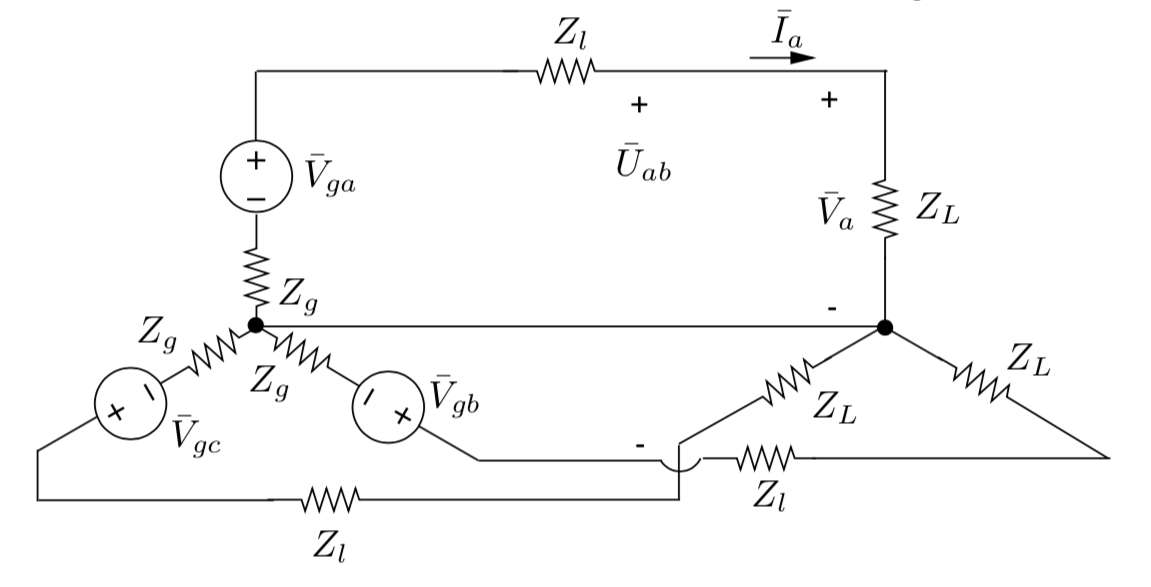
\includegraphics[width=0.72\linewidth]{../Lectures/ThreePhaseAndPu/images/three-phase-system.png}
        \caption{Balanced wye-connected three-phase source and load system.}
        \label{fig:tp2_wye}
    \end{figure}
\end{enumerate}

\newpage
\subsection{Solutions}

\subsubsection*{Solution to Exercise 1: Three-Phase Source Phasors and Waveforms}
\paragraph{Data:}
Positive sequence ($a$-$b$-$c$) balanced source with:
\[
\bar{V}_a = \sqrt{2} \times 100 e^{j 30^\circ}\ \text{V} = 141.42\ \text{V} \angle 30^\circ = 122.47 + j70.71\ \text{V}
\]
Since the phasor is given in RMS, the amplitude of the time-domain sinusoidal wave is $\sqrt{2} \times |\bar{V}_a| = \sqrt{2} \times 141.42 = 200\ \text{V}$.

\paragraph{Time-Domain Voltages:}
\begin{align}
    \boxed{v_a(t) = 200 \cos(\omega t + 30^\circ)\ \text{V}}
\end{align}
In a balanced positive-sequence system, phase $b$ lags phase $a$ by $120^\circ$, and phase $c$ leads phase $a$ by $120^\circ$ (or lags by $240^\circ$):
\begin{align}
    \bar{V}_b &= \bar{V}_a e^{-j 120^\circ} = \sqrt{2} \times 100 e^{j (30^\circ - 120^\circ)} \nonumber\\
              &= \sqrt{2} \times 100 e^{-j 90^\circ} = -j 141.42\ \text{V} \\
    \boxed{v_b(t) = 200 \cos(\omega t - 90^\circ)\ \text{V}}
\end{align}
\begin{align}
    \bar{V}_c &= \bar{V}_a e^{+j 120^\circ} = \sqrt{2} \times 100 e^{j (30^\circ + 120^\circ)} \nonumber\\
              &= \sqrt{2} \times 100 e^{j 150^\circ} = -122.47 + j 70.71\ \text{V} \\
    \boxed{v_c(t) = 200 \cos(\omega t + 150^\circ)\ \text{V}}
\end{align}

\paragraph{Line-to-Line Voltage $\bar{V}_{ab}$:}
\begin{align}
    \bar{V}_{ab} &= \bar{V}_a - \bar{V}_b = \sqrt{2} \times 100 \left( e^{j 30^\circ} - e^{-j 90^\circ} \right) \nonumber\\
                 &= (122.47 + j 70.71) - (-j 141.42) = 122.47 + j 212.13\ \text{V} \nonumber\\
                 &= 244.95\ \text{V} \angle 60^\circ = \sqrt{3} \bar{V}_a e^{j 30^\circ}
\end{align}
The peak amplitude is $200 \sqrt{3} = 346.41\ \text{V}$:
\begin{equation}
    \boxed{v_{ab}(t) = 200\sqrt{3} \cos(\omega t + 60^\circ)\ \text{V} = 346.41 \cos(\omega t + 60^\circ)\ \text{V}}
\end{equation}

\begin{figure}[htbp]
    \centering
    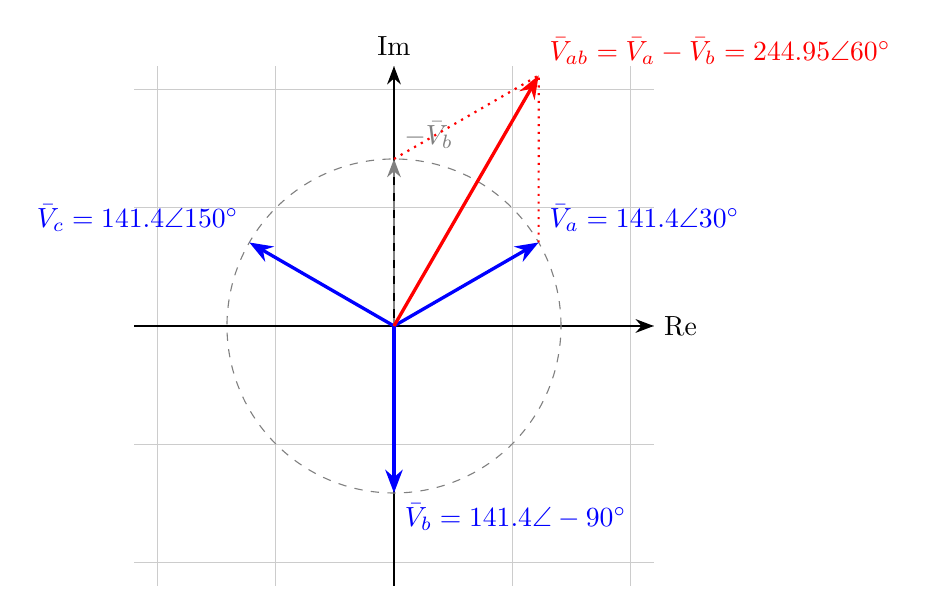
\begin{tikzpicture}[scale=1.5, >=Stealth]
        % Axes
        \draw[thin, gray!40] (-2.2,-2.2) grid (2.2,2.2);
        \draw[->, thick] (-2.2,0) -- (2.2,0) node[right] {$\text{Re}$};
        \draw[->, thick] (0,-2.2) -- (0,2.2) node[above] {$\text{Im}$};
        \draw[dashed, gray] (0,0) circle (1.414);

        % Phasors
        \draw[->, very thick, blue] (0,0) -- (30:1.414) node[above right] {$\bar{V}_a = 141.4\angle 30^\circ$};
        \draw[->, very thick, blue] (0,0) -- (-90:1.414) node[below right] {$\bar{V}_b = 141.4\angle -90^\circ$};
        \draw[->, very thick, blue] (0,0) -- (150:1.414) node[above left] {$\bar{V}_c = 141.4\angle 150^\circ$};
        \draw[->, dashed, thick, gray] (0,0) -- (90:1.414) node[above right] {$-\bar{V}_b$};

        % Line-to-line Vab
        \draw[->, very thick, red] (0,0) -- (60:2.45) node[above right] {$\bar{V}_{ab} = \bar{V}_a - \bar{V}_b = 244.95\angle 60^\circ$};
        \draw[dotted, thick, red] (30:1.414) -- (60:2.45);
        \draw[dotted, thick, red] (90:1.414) -- (60:2.45);
    \end{tikzpicture}
    \caption{Phasor diagram of balanced phase voltages and line-to-line voltage $\bar{V}_{ab}$.}
    \label{fig:tp2_phasor1}
\end{figure}

\subsubsection*{Solution to Exercise 2: Balanced Three-Phase Inductive Load}
\paragraph{Data:}
\begin{itemize}
    \item Phase voltage: $V_{1\phi} = 120\ \text{V}$ RMS
    \item Total 3-phase active power: $P_{3\phi} = 10\ \text{kW} = 10^4\ \text{W}$
    \item Power factor: $\cos\phi = 0.9$ (inductive/lagging) $\implies \phi = +\arccos(0.9) = +25.842^\circ$
\end{itemize}

\paragraph{1. Phase Current RMS Value:}
The per-phase active power is:
\[
P_{1\phi} = \frac{P_{3\phi}}{3} = \frac{10^4}{3} = 3333.33\ \text{W}
\]
Using $P_{1\phi} = V_{1\phi} I_{\text{RMS}} \cos\phi$:
\begin{equation}
    \boxed{I_{\text{RMS}} = \frac{P_{1\phi}}{V_{1\phi} \cos\phi} = \frac{3333.33}{120 \times 0.9} = 30.86\ \text{A}}
\end{equation}

\paragraph{2. Load Impedance $Z_{1\phi}$:}
For a wye connection, the voltage across each phase impedance is the phase voltage $V_{1\phi} = 120\ \text{V}$:
\begin{equation}
    |Z_{1\phi}| = \frac{V_{1\phi}}{I_{\text{RMS}}} = \frac{120}{30.864} = 3.888\ \Omega
\end{equation}
Since the load is inductive, current lags voltage by $\phi = 25.84^\circ$, meaning the impedance angle is positive:
\begin{equation}
    \boxed{Z_{1\phi} = 3.888\ \Omega \angle +25.84^\circ = (3.50 + j1.70)\ \Omega}
\end{equation}

\paragraph{3. Phasor Diagram:}
Taking $\bar{V}_a = 120\angle 0^\circ\ \text{V}$ as reference:
\begin{itemize}
    \item Voltages: $\bar{V}_a = 120\angle 0^\circ\ \text{V}$, $\bar{V}_b = 120\angle -120^\circ\ \text{V}$, $\bar{V}_c = 120\angle +120^\circ\ \text{V}$
    \item Currents: $\bar{I}_a = 30.86\ \text{A} \angle -25.84^\circ$, $\bar{I}_b = 30.86\ \text{A} \angle -145.84^\circ$, $\bar{I}_c = 30.86\ \text{A} \angle +94.16^\circ$
\end{itemize}

\begin{figure}[htbp]
    \centering
    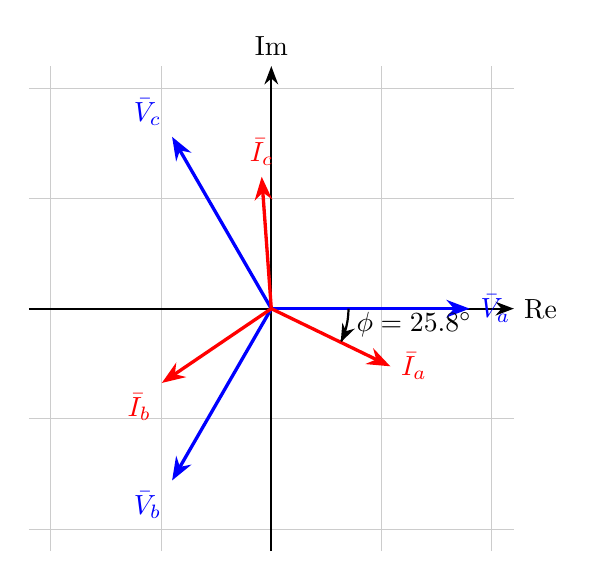
\begin{tikzpicture}[scale=1.4, >=Stealth]
        \draw[thin, gray!40] (-2.2,-2.2) grid (2.2,2.2);
        \draw[->, thick] (-2.2,0) -- (2.2,0) node[right] {$\text{Re}$};
        \draw[->, thick] (0,-2.2) -- (0,2.2) node[above] {$\text{Im}$};

        % Voltages (scaled to length 1.8)
        \draw[->, very thick, blue] (0,0) -- (0:1.8) node[right] {$\bar{V}_a$};
        \draw[->, very thick, blue] (0,0) -- (-120:1.8) node[below left] {$\bar{V}_b$};
        \draw[->, very thick, blue] (0,0) -- (120:1.8) node[above left] {$\bar{V}_c$};

        % Currents (scaled to length 1.2)
        \draw[->, very thick, red] (0,0) -- (-25.84:1.2) node[right] {$\bar{I}_a$};
        \draw[->, very thick, red] (0,0) -- (-145.84:1.2) node[below left] {$\bar{I}_b$};
        \draw[->, very thick, red] (0,0) -- (94.16:1.2) node[above] {$\bar{I}_c$};

        % Angle arc
        \draw[->, thick, domain=0:-25.84] plot ({0.7*cos(\x)}, {0.7*sin(\x)});
        \node[right] at (-12:0.7) {$\phi = 25.8^\circ$};
    \end{tikzpicture}
    \caption{Phasor diagram of voltages and lagging currents for the balanced inductive load.}
    \label{fig:tp2_phasor2}
\end{figure}

\subsubsection*{Solution to Exercise 3: Power Transfer Between Two AC Systems}
\paragraph{Data:}
\begin{itemize}
    \item Transferred active power: $P = 1\ \text{kW} = 1000\ \text{W}$
    \item Sending-end voltage: $V_S = 100\ \text{V}$ (angle $\theta_S$ to be determined)
    \item Receiving-end voltage: $\bar{V}_R = 95\ \text{V}\angle 0^\circ \implies V_R = 95\ \text{V}$, $\theta_R = 0^\circ$
    \item Line reactance: $X = 1.5\ \Omega$ (lossless line, $R = 0$)
\end{itemize}

\paragraph{Derivation of Power Transfer Formulas:}
The line current directed from $S$ to $R$ is:
\begin{equation}
    \bar{I} = \frac{\bar{V}_S - \bar{V}_R}{jX}
\end{equation}
The complex power injected by the sending-end source $S$ is:
\begin{align}
    S_S &= \bar{V}_S \bar{I}^* = \bar{V}_S \left(\frac{\bar{V}_S - \bar{V}_R}{jX}\right)^* = \frac{V_S^2 - \bar{V}_S \bar{V}_R^*}{-jX} = j \frac{V_S^2 - V_S V_R e^{j(\theta_S - \theta_R)}}{X} \nonumber\\
        &= \frac{V_S V_R \sin(\theta_S - \theta_R)}{X} + j \frac{V_S^2 - V_S V_R \cos(\theta_S - \theta_R)}{X}
\end{align}
Hence:
\begin{align}
    P_S &= \frac{V_S V_R \sin(\theta_S - \theta_R)}{X} \label{eq:PS_formula}\\
    Q_S &= \frac{V_S^2 - V_S V_R \cos(\theta_S - \theta_R)}{X} \label{eq:QS_formula}
\end{align}

\paragraph{Phase Angle $\theta_S$:}
Since the line is lossless ($R = 0$), $P_S = P_R = 1000\ \text{W}$. With $\theta_R = 0^\circ$:
\begin{equation}
    \sin\theta_S = \frac{X P_S}{V_S V_R} = \frac{1.5 \times 1000}{100 \times 95} = \frac{1500}{9500} = 0.15789
\end{equation}
\begin{equation}
    \boxed{\theta_S = \arcsin(0.15789) = 9.085^\circ\quad (0.1585\ \text{rad})}
\end{equation}

\paragraph{Line Current $\bar{I}$:}
\begin{align}
    \bar{I} &= \frac{100\angle 9.085^\circ - 95\angle 0^\circ}{j 1.5} = \frac{(98.743 + j15.789) - 95}{j 1.5} \nonumber\\
            &= \frac{3.743 + j15.789}{j 1.5} = \frac{15.789 - j3.743}{1.5} = 10.526 - j2.495\ \text{A} \nonumber\\
            &= \boxed{10.818\ \text{A} \angle -13.35^\circ}
\end{align}

\paragraph{Per-Phase Reactive Power $Q_R$ Supplied to the Receiving End:}
The power received at bus $R$ is:
\begin{align}
    S_R &= \bar{V}_R \bar{I}^* = (95\angle 0^\circ)(10.526 + j2.495) \nonumber\\
        &= 999.97 + j237.06\ \text{VA} \approx 1000\ \text{W} + j 237.22\ \text{var}
\end{align}
Alternatively, using the analytical receiving-end formula:
\begin{align}
    Q_R &= \text{Im}\{\bar{V}_R \bar{I}^*\} = \frac{V_S V_R \cos(\theta_R - \theta_S) - V_R^2}{X} \nonumber\\
        &= \frac{100 \times 95 \times \cos(-9.085^\circ) - 95^2}{1.5} \nonumber\\
        &= \frac{9500 \times 0.9874 - 9025}{1.5} = \frac{9380.57 - 9025}{1.5} = \boxed{237.05\ \text{var} \approx 237.22\ \text{var}}
\end{align}
\textit{Note on sign convention:} As annotated in the handwritten notes, $Q_R > 0$ indicates that the line supplies $237.22\ \text{var}$ of reactive power into the receiving-end source/bus.

\subsubsection*{Solution to Exercise 4: Voltage Profile of a Radial Transmission System}
\paragraph{(a) Load Reactive Power $Q_R$:}
Let the load complex power be $S_R = P_R + j Q_R$. By definition of the load power factor:
\begin{equation}
    \cos\phi = \frac{P_R}{|S_R|} = \frac{P_R}{\sqrt{P_R^2 + Q_R^2}} \iff Q_R = \pm P_R \sqrt{\frac{1}{\cos^2\phi} - 1}
\end{equation}
\begin{itemize}
    \item \textbf{Unity power factor ($\cos\phi = 1$):} $Q_R = 0$.
    \item \textbf{Lagging power factor ($\cos\phi = 0.9$):} $Q_R = + P_R \sqrt{\frac{1}{0.9^2} - 1} = +0.4843 P_R > 0$ (inductive load consumes reactive power).
    \item \textbf{Leading power factor ($\cos\phi = 0.9$):} $Q_R = - P_R \sqrt{\frac{1}{0.9^2} - 1} = -0.4843 P_R < 0$ (capacitive load generates reactive power).
\end{itemize}

\paragraph{(b) Second-Order Equation for $V_R^2$:}
Let $\delta = \theta_R - \theta_S$ be the transmission angle. The power flow equations at the receiving end are:
\begin{align}
    P_R &= \frac{V_S V_R \sin\delta}{X} \implies V_R \sin\delta = \frac{P_R X}{V_S} \label{eq:radial_sin}\\
    Q_R &= \frac{V_S V_R \cos\delta - V_R^2}{X} \implies V_R \cos\delta = \frac{X Q_R + V_R^2}{V_S} \label{eq:radial_cos}
\end{align}
Squaring and summing equations~\eqref{eq:radial_sin} and~\eqref{eq:radial_cos}:
\begin{equation}
    V_R^2 (\sin^2\delta + \cos^2\delta) = V_R^2 = \left(\frac{P_R X}{V_S}\right)^2 + \left(\frac{X Q_R + V_R^2}{V_S}\right)^2
\end{equation}
Multiplying both sides by $V_S^2$:
\begin{equation}
    V_S^2 V_R^2 = P_R^2 X^2 + X^2 Q_R^2 + 2 X Q_R V_R^2 + V_R^4
\end{equation}
Rearranging terms into standard polynomial form in $y = V_R^2$:
\begin{equation}
    \boxed{y^2 + (2X Q_R - V_S^2) y + X^2 (P_R^2 + Q_R^2) = 0\quad \text{with}\quad y = V_R^2}
\end{equation}

\paragraph{(c) Ratio $V_S/V_R$ and Power Angle $\delta$:}
Solving the quadratic equation for $y = V_R^2$:
\begin{equation}
    V_R^2 = \frac{-(2X Q_R - V_S^2) + \sqrt{(2X Q_R - V_S^2)^2 - 4 X^2(P_R^2 + Q_R^2)}}{2}
\end{equation}
(choosing the positive square root corresponding to normal, stable operating voltage).
Once $V_R$ is obtained, the power angle $\delta$ is:
\begin{equation}
    \delta = \arcsin\left(\frac{P_R X}{V_S V_R}\right)
\end{equation}

\paragraph{Physical Interpretation:}
\begin{itemize}
    \item \textbf{Lagging power factor (inductive):} As $P_R$ increases, the line reactive drop adds to the load reactive demand, causing a severe drop in receiving voltage $V_R$, so $V_S/V_R > 1$ increases rapidly.
    \item \textbf{Unity power factor:} $V_R$ exhibits a moderate voltage drop due to the line series reactance.
    \item \textbf{Leading power factor (capacitive):} The capacitive reactive power supports the voltage (Ferranti-like compensation effect), keeping $V_R$ elevated ($V_S/V_R \approx 1$ or even $< 1$ for light loads).
\end{itemize}

\subsubsection*{Solution to Exercise 5: Per-Unit Analysis of a Three-Phase System}
\paragraph{Data:}
\begin{itemize}
    \item Impedance magnitude: $|Z_L| = 10\ \Omega$
    \item Power factor: $\cos\phi = 0.8$ lagging $\implies \phi = \arccos(0.8) = +36.87^\circ$
    \item Load impedance: $Z_L = 10\ \Omega \angle 36.87^\circ = (8 + j6)\ \Omega$
\end{itemize}

\paragraph{Per-Unit Formulas:}
\begin{itemize}
    \item Phase voltage base: $V^B = \frac{U^B}{\sqrt{3}}$
    \item Single-phase power base: $S_{1\phi}^B = \frac{S_{3\phi}^B}{3}$
    \item Current base: $I^B = \frac{S_{1\phi}^B}{V^B} = \frac{S_{3\phi}^B}{\sqrt{3} U^B}$
    \item Base impedance: $Z^B = \frac{(V^B)^2}{S_{1\phi}^B} = \frac{(U^B)^2}{S_{3\phi}^B}$
\end{itemize}

\paragraph{Detailed Calculations for the Three Base Systems:}
\begin{table}[htbp]
    \centering
    \caption{Base quantities and per-unit values for Exercise 5.}
    \label{tab:tp2_pu}
    \renewcommand{\arraystretch}{1.3}
    \begin{tabular}{lccc}
        \toprule
        \textbf{Quantity} & \textbf{Case (a)} & \textbf{Case (b)} & \textbf{Case (c)} \\
        \midrule
        $U^B$ (line-to-line) & $208\ \text{V}$ & $240\ \text{V}$ & $240\ \text{V}$ \\
        $S_{3\phi}^B$ & $3.6\ \text{kVA}$ & $5.4\ \text{kVA}$ & $3.6\ \text{kVA}$ \\
        \midrule
        $V^B = U^B / \sqrt{3}$ & $120.09\ \text{V}$ & $138.56\ \text{V}$ & $138.56\ \text{V}$ \\
        $S_{1\phi}^B = S_{3\phi}^B / 3$ & $1.2\ \text{kVA}$ & $1.8\ \text{kVA}$ & $1.2\ \text{kVA}$ \\
        $I^B = S_{1\phi}^B / V^B$ & $10.0\ \text{A}$ & $13.0\ \text{A}$ & $8.66\ \text{A}$ \\
        $Z^B = (U^B)^2 / S_{3\phi}^B$ & $12.018\ \Omega$ & $10.667\ \Omega$ & $16.000\ \Omega$ \\
        \midrule
        $|Z_{L,pu}| = |Z_L| / Z^B$ & $0.832\ \text{pu}$ & $0.9375\ \text{pu}$ & $0.625\ \text{pu}$ \\
        $Z_{L,pu}$ & $\mathbf{0.832\angle 36.87^\circ\ \text{pu}}$ & $\mathbf{0.938\angle 36.87^\circ\ \text{pu}}$ & $\mathbf{0.625\angle 36.87^\circ\ \text{pu}}$ \\
        \midrule
        $|S_{1\phi}| = (V^B)^2 / |Z_L|$ & $1442.13\ \text{VA}$ & $1920.0\ \text{VA}$ & $1920.0\ \text{VA}$ \\
        $P_{1\phi} = |S_{1\phi}|\cos\phi$ & $1153.71\ \text{W}$ & $1536.0\ \text{W}$ & $1536.0\ \text{W}$ \\
        $Q_{1\phi} = |S_{1\phi}|\sin\phi$ & $865.28\ \text{var}$ & $1152.0\ \text{var}$ & $1152.0\ \text{var}$ \\
        \midrule
        $P_{pu} = P_{1\phi} / S_{1\phi}^B$ & $\mathbf{0.9614\ \text{pu}}$ & $\mathbf{0.8533\ \text{pu}}$ & $\mathbf{1.2800\ \text{pu}}$ \\
        $Q_{pu} = Q_{1\phi} / S_{1\phi}^B$ & $\mathbf{0.7213\ \text{pu}}$ & $\mathbf{0.6400\ \text{pu}}$ & $\mathbf{0.9600\ \text{pu}}$ \\
        \bottomrule
    \end{tabular}
\end{table}
Notice that in per-unit:
\[
S_{pu} = \frac{|V_{pu}|^2}{Z_{L,pu}^*} = \frac{1}{Z_{L,pu}^*} = \frac{1}{|Z_{L,pu}|} \angle 36.87^\circ
\]
For example, in case (a): $|S_{pu}| = 1 / 0.832 = 1.2018\ \text{pu}$, giving $P_{pu} = 1.2018 \times 0.8 = 0.9614\ \text{pu}$ and $Q_{pu} = 1.2018 \times 0.6 = 0.7211\ \text{pu}$, which matches perfectly.

\newpage

\section{Practical Session 3: The Transmission Line}

\subsection{Exercises}
\begin{enumerate}
    \item \textbf{Surge Impedance Loading (SIL) and Line Losses}\footnote{Exercises 4.3 and 4.10 of Ned Mohan's book \textit{"Electric power systems, a first course"}.}
    
    The parameters for a $500\text{-kV}$ transmission system with bundled conductors are as follows:
    \[
    Z_c = 258\ \Omega,\quad R = 1.76 \times 10^{-2}\ \Omega/\text{km}.
    \]
    \begin{enumerate}
        \item Demonstrate why the voltage magnitude along a lossless line terminated in its surge impedance $Z_c$ is constant.
        \item Calculate the Surge Impedance Loading (SIL) of the transmission system.
        \item Calculate the percentage active power loss in this transmission line if it is $300\ \text{km}$ long and operates loaded at its SIL.
    \end{enumerate}

    \item \textbf{Distributed-Parameter Line Model and Voltage Profiles}
    
    Table~\ref{tab:tp3_params} gives approximate transmission line parameters with bundled conductors at $60\ \text{Hz}$.
    
    \begin{table}[htbp]
        \centering
        \caption{Approximate transmission line parameters with bundled conductors at $60\ \text{Hz}$.}
        \label{tab:tp3_params}
        \renewcommand{\arraystretch}{1.2}
        \begin{tabular}{cccc}
            \toprule
            \textbf{Nominal voltage} [$\text{kV}$] & $R$ [$\Omega/\text{km}$] & $\omega L$ [$\Omega/\text{km}$] & $\omega C$ [$\mu\text{S/km}$] \\
            \midrule
            $230$ & $0.06$ & $0.50$ & $3.4$ \\
            $345$ & $0.04$ & $0.38$ & $4.6$ \\
            $500$ & $0.03$ & $0.33$ & $5.3$ \\
            $765$ & $0.01$ & $0.34$ & $5.0$ \\
            \bottomrule
        \end{tabular}
    \end{table}

    A $200\ \text{km}$ long $345\text{-kV}$ line has the parameters given in Table~\ref{tab:tp3_params}. Neglect the line series resistance ($R = 0$).
    \begin{enumerate}
        \item Starting from an infinitesimal section of length $dx$ (Figure~\ref{fig:tp3_distributed}), derive the Telegrapher's wave equations in the time domain, and then convert them into the phasor domain.
        \item Solve the differential equations in terms of the receiving-end boundary conditions $\bar{V}_R$ and $\bar{I}_R$.
        \item Calculate the voltage profile along the line if the receiving end is held at $1.0\ \text{pu}$ ($V_R = 345\ \text{kV}$) with $\cos\phi = 1.0$, for:
        \begin{enumerate}[(a)]
            \item A load of $1.5 \times \text{SIL}$
            \item A load of $0.75 \times \text{SIL}$
        \end{enumerate}
        Evaluate the voltage magnitude at $x = 100\ \text{km}$ and at the sending end $x = 200\ \text{km}$.
    \end{enumerate}

    \begin{figure}[htbp]
        \centering
        \begin{circuitikz}[american, scale=1.1]
            \draw (0,2) coordinate (in_top)
                  -- ++(1.5,0)
                  to[L, l=$dL{=}L\,dx$, i=$i(x{,}t)$] ++(2.5,0)
                  -- ++(1.5,0) coordinate (out_top);
            \draw (1.5,2) to[C, l=$dC/2$] ++(0,-2) coordinate (in_bot);
            \draw (4.0,2) to[C, l=$dC/2$] ++(0,-2) coordinate (out_bot);
            \draw (in_bot) -- (out_bot);
            
            % Labels
            \node[above] at (in_top) {$v(x-dx{,}t)$};
            \node[above] at (out_top) {$v(x+dx{,}t)$};
            \draw[<->] (1.5,-0.5) -- (4.0,-0.5) node[midway, below] {$dx$};
        \end{circuitikz}
        \caption{Infinitesimal section $dx$ of a lossless distributed transmission line.}
        \label{fig:tp3_distributed}
    \end{figure}
\end{enumerate}

\newpage
\subsection{Solutions}

\subsubsection*{Solution to Exercise 1: Surge Impedance Loading (SIL) and Losses}
\paragraph{Data:}
\begin{itemize}
    \item Rated line-to-line voltage: $V_{LL} = 500\ \text{kV}$
    \item Surge impedance: $Z_c = 258\ \Omega$
    \item Resistance per unit length: $R = 1.76 \times 10^{-2}\ \Omega/\text{km}$
    \item Line length: $l = 300\ \text{km}$
\end{itemize}

\paragraph{1. Voltage Flatness at SIL Termination:}
The general expression for the voltage phasor at a distance $x$ from the receiving end on a lossless transmission line is:
\begin{equation}
    \bar{V}(x) = \bar{V}_R \cos(\beta x) + j Z_c \bar{I}_R \sin(\beta x) \label{eq:lossless_V_profile}
\end{equation}
When the line is terminated by its characteristic impedance $Z_c$ under a resistive load ($\bar{V}_R = V_R \angle 0^\circ$ and $\cos\phi = 1$), the receiving-end current is:
\begin{equation}
    \bar{I}_R = \frac{\bar{V}_R}{Z_c}
\end{equation}
Substituting this into~\eqref{eq:lossless_V_profile}:
\begin{equation}
    \bar{V}(x) = \bar{V}_R \cos(\beta x) + j Z_c \left(\frac{\bar{V}_R}{Z_c}\right) \sin(\beta x) = \bar{V}_R \left( \cos(\beta x) + j\sin(\beta x) \right) = \bar{V}_R e^{j \beta x}
\end{equation}
Taking the magnitude:
\begin{equation}
    |\bar{V}(x)| = |\bar{V}_R| = \text{constant} \quad \forall x
\end{equation}
Thus, the voltage magnitude remains strictly constant along the entire length of the line: only the phase angle advances linearly with $x$ by $\beta x$.

\paragraph{2. Surge Impedance Loading (SIL):}
By definition, the Surge Impedance Loading is the total three-phase active power delivered into a load equal to the surge impedance $Z_c$ at nominal voltage:
\begin{equation}
    \boxed{\text{SIL} = \frac{V_{LL}^2}{Z_c} = \frac{(500 \times 10^3)^2}{258} = 9.6899 \times 10^8\ \text{W} \approx 969\ \text{MW}}
\end{equation}

\paragraph{3. Percentage Power Loss for $l = 300\ \text{km}$:}
At rated SIL, the equivalent line current is:
\begin{equation}
    I = \frac{\text{SIL}}{V_{LL}} = \frac{968.99 \times 10^6\ \text{W}}{500 \times 10^3\ \text{V}} = 1937.98\ \text{A}
\end{equation}
The total resistance of the line is:
\begin{equation}
    R_{\text{tot}} = R \cdot l = (1.76 \times 10^{-2}\ \Omega/\text{km}) \times 300\ \text{km} = 5.28\ \Omega
\end{equation}
The Joule losses in the line are:
\begin{equation}
    P_{\text{loss}} = R_{\text{tot}} I^2 = 5.28 \times (1937.98)^2 = 19.831 \times 10^6\ \text{W} = 19.831\ \text{MW}
\end{equation}
The relative percentage loss is:
\begin{equation}
    \boxed{\%\ \text{loss} = \frac{P_{\text{loss}}}{\text{SIL}} \times 100 = \frac{19.831\ \text{MW}}{968.99\ \text{MW}} \times 100 = 2.05\%}
\end{equation}

\subsubsection*{Solution to Exercise 2: Distributed Line Model and Voltage Profile}
\paragraph{Data for $345\text{-kV}$ Line:}
\begin{itemize}
    \item Rated voltage: $V_{LL} = 345\ \text{kV} = 3.45 \times 10^5\ \text{V}$
    \item Length: $l = 200\ \text{km}$
    \item Series reactance per unit length: $\omega L = 0.38\ \Omega/\text{km}$
    \item Shunt susceptance per unit length: $\omega C = 4.6\ \mu\text{S/km} = 4.6 \times 10^{-6}\ \text{S/km}$
    \item Line resistance: $R = 0$ (lossless line assumption)
\end{itemize}

\paragraph{Characteristic Parameters:}
\begin{itemize}
    \item Surge impedance:
    \begin{equation}
        Z_c = \sqrt{\frac{L}{C}} = \sqrt{\frac{\omega L}{\omega C}} = \sqrt{\frac{0.38}{4.6 \times 10^{-6}}} = 287.417\ \Omega
    \end{equation}
    \item Phase propagation constant:
    \begin{equation}
        \beta = \omega \sqrt{LC} = \sqrt{(\omega L)(\omega C)} = \sqrt{0.38 \times 4.6 \times 10^{-6}} = 1.322 \times 10^{-3}\ \text{rad/km} = 0.001322\ \text{rad/km}
    \end{equation}
    \item Surge Impedance Loading:
    \begin{equation}
        \text{SIL} = \frac{V_{LL}^2}{Z_c} = \frac{(345 \times 10^3)^2}{287.417} = 4.1412 \times 10^8\ \text{VA} = 414.12\ \text{MVA (MW)}
    \end{equation}
\end{itemize}

\paragraph{1. Derivation of Telegrapher's Equations:}
Consider an infinitesimal line slice of length $dx$ with distributed inductance $L$ and capacitance $C$ per unit length.
Applying Kirchhoff's Current Law (KCL):
\begin{align}
    i(x - dx, t) &= i(x, t) + (C\,dx) \frac{\partial v(x, t)}{\partial t} \nonumber\\
    \iff \frac{i(x, t) - i(x - dx, t)}{dx} &= - C \frac{\partial v(x, t)}{\partial t}
\end{align}
Taking the limit as $dx \to 0$:
\begin{equation}
    -\frac{\partial i(x, t)}{\partial x} = C \frac{\partial v(x, t)}{\partial t} \label{eq:kcl_telegraph}
\end{equation}

Applying Kirchhoff's Voltage Law (KVL):
\begin{align}
    v(x, t) &= (L\,dx) \frac{\partial i(x, t)}{\partial t} + v(x + dx, t) \nonumber\\
    \iff \frac{v(x + dx, t) - v(x, t)}{dx} &= - L \frac{\partial i(x, t)}{\partial t}
\end{align}
Taking the limit as $dx \to 0$:
\begin{equation}
    -\frac{\partial v(x, t)}{\partial x} = L \frac{\partial i(x, t)}{\partial t} \label{eq:kvl_telegraph}
\end{equation}

Equations~\eqref{eq:kcl_telegraph} and~\eqref{eq:kvl_telegraph} are the celebrated \textbf{Telegrapher's equations} in the time domain.
Differentiating~\eqref{eq:kcl_telegraph} with respect to $x$ and~\eqref{eq:kvl_telegraph} with respect to $t$:
\begin{align}
    -\frac{\partial^2 i}{\partial x^2} &= C \frac{\partial^2 v}{\partial x \partial t} \\
    -\frac{\partial^2 v}{\partial t \partial x} &= L \frac{\partial^2 i}{\partial t^2}
\end{align}
Substituting:
\begin{equation}
    \boxed{\frac{\partial^2 i(x, t)}{\partial x^2} = L C \frac{\partial^2 i(x, t)}{\partial t^2}} \label{eq:wave_i}
\end{equation}
Similarly for the voltage:
\begin{equation}
    \boxed{\frac{\partial^2 v(x, t)}{\partial x^2} = L C \frac{\partial^2 v(x, t)}{\partial t^2}} \label{eq:wave_v}
\end{equation}

\paragraph{Phasor Domain Representation:}
Under sinusoidal steady state, $\frac{\partial}{\partial t} \to j\omega$ and $\frac{\partial^2}{\partial t^2} \to -\omega^2$. Equation~\eqref{eq:wave_i} becomes:
\begin{equation}
    \frac{d^2 \bar{I}(x)}{dx^2} + \omega^2 L C \bar{I}(x) = 0 \iff \frac{d^2 \bar{I}(x)}{dx^2} + \beta^2 \bar{I}(x) = 0 \label{eq:phasor_diff_eq}
\end{equation}
where $\beta = \omega\sqrt{LC}$. The general solution of this linear second-order differential equation is:
\begin{equation}
    \bar{I}(x) = I_1 e^{j \beta x} + I_2 e^{-j \beta x} \label{eq:I_general}
\end{equation}
From~\eqref{eq:kcl_telegraph} in the phasor domain:
\begin{align}
    -\frac{d\bar{I}(x)}{dx} = j\omega C \bar{V}(x) \implies \bar{V}(x) &= -\frac{1}{j\omega C} \frac{d\bar{I}(x)}{dx} \nonumber\\
    &= -\frac{1}{j\omega C} \left( j\beta I_1 e^{j\beta x} - j\beta I_2 e^{-j\beta x} \right) \nonumber\\
    &= -\frac{\beta}{\omega C} \left( I_1 e^{j\beta x} - I_2 e^{-j\beta x} \right)
\end{align}
Since $\frac{\beta}{\omega C} = \frac{\omega\sqrt{LC}}{\omega C} = \sqrt{\frac{L}{C}} = Z_c$:
\begin{equation}
    \bar{V}(x) = Z_c \left( -I_1 e^{j\beta x} + I_2 e^{-j\beta x} \right) \label{eq:V_general}
\end{equation}

\paragraph{2. Boundary Conditions at Receiving End ($x = 0$):}
At the receiving end $x = 0$, let $\bar{V}(0) = \bar{V}_R$ and $\bar{I}(0) = \bar{I}_R$:
\begin{equation}
\begin{cases}
    \bar{V}_R = Z_c (-I_1 + I_2) \\
    \bar{I}_R = I_1 + I_2
\end{cases}
\iff
\begin{cases}
    -I_1 + I_2 = \frac{\bar{V}_R}{Z_c} \\
    I_1 + I_2 = \bar{I}_R
\end{cases}
\end{equation}
Solving for $I_1$ and $I_2$:
\begin{align}
    I_1 &= \frac{\bar{I}_R - \bar{V}_R/Z_c}{2} \label{eq:I1_const}\\
    I_2 &= \frac{\bar{I}_R + \bar{V}_R/Z_c}{2} \label{eq:I2_const}
\end{align}
Substituting~\eqref{eq:I1_const} and~\eqref{eq:I2_const} into~\eqref{eq:V_general}:
\begin{align}
    \bar{V}(x) &= Z_c \left[ -\left(\frac{\bar{I}_R - \bar{V}_R/Z_c}{2}\right) e^{j\beta x} + \left(\frac{\bar{I}_R + \bar{V}_R/Z_c}{2}\right) e^{-j\beta x} \right] \nonumber\\
               &= \bar{V}_R \left( \frac{e^{j\beta x} + e^{-j\beta x}}{2} \right) - Z_c \bar{I}_R \left( \frac{e^{j\beta x} - e^{-j\beta x}}{2} \right) \nonumber\\
               &= \boxed{\bar{V}(x) = \bar{V}_R \cos(\beta x) + j Z_c \bar{I}_R \sin(\beta x)} \label{eq:voltage_profile_final}
\end{align}
and similarly:
\begin{equation}
    \boxed{\bar{I}(x) = \bar{I}_R \cos(\beta x) + j \frac{\bar{V}_R}{Z_c} \sin(\beta x)}
\end{equation}

\paragraph{3. Voltage Profiles for Loading Conditions:}
At the receiving end, the voltage is held at nominal 1 pu:
\[
\bar{V}_R = 3.45 \times 10^5\angle 0^\circ\ \text{V}.
\]
The load operates at unity power factor ($\cos\phi = 1.0$), so $\bar{I}_R = I_R \angle 0^\circ$.
\begin{enumerate}[(a)]
    \item \textbf{Heavy loading ($1.5 \times \text{SIL}$):}
    \[
    P_L = 1.5 \times 414.12\ \text{MW} = 621.18\ \text{MW}
    \]
    \[
    \bar{I}_R = \frac{P_L}{V_R} = \frac{621.18 \times 10^6\ \text{W}}{3.45 \times 10^5\ \text{V}} = 1800.518\ \text{A}\angle 0^\circ
    \]
    
    \item \textbf{Light loading ($0.75 \times \text{SIL}$):}
    \[
    P_L = 0.75 \times 414.12\ \text{MW} = 312.059\ \text{MW}
    \]
    \[
    \bar{I}_R = \frac{P_L}{V_R} = \frac{312.059 \times 10^6\ \text{W}}{3.45 \times 10^5\ \text{V}} = 900.259\ \text{A}\angle 0^\circ
    \]
\end{enumerate}

\paragraph{Numerical Evaluation along the Line (for Case a: $1.5 \times \text{SIL}$):}
\begin{itemize}
    \item At $x = 0$ (receiving end):
    \[
    \bar{V}(0) = \bar{V}_R = 345.0\ \text{kV}\angle 0^\circ \quad (1.000\ \text{pu})
    \]
    
    \item At $x = 100\ \text{km}$:
    \[
    \beta x = (0.001322\ \text{rad/km}) \times 100\ \text{km} = 0.1322\ \text{rad} = 7.574^\circ
    \]
    \[
    \cos(\beta x) = \cos(0.1322\ \text{rad}) = 0.99128,\quad \sin(\beta x) = \sin(0.1322\ \text{rad}) = 0.13182
    \]
    Substituting into~\eqref{eq:voltage_profile_final}:
    \begin{align}
        \bar{V}(100\ \text{km}) &= (3.45 \times 10^5)(0.99128) + j (287.417 \times 1800.518)(0.13182) \nonumber\\
                                &= 341.99 \times 10^3 + j 68.22 \times 10^3\ \text{V} \nonumber\\
                                &= 3.4872 \times 10^5\ \text{V} \angle 11.28^\circ \quad (1.0108\ \text{pu})
    \end{align}
    \begin{equation}
        \boxed{|\bar{V}(100\ \text{km})| \approx 3.49 \times 10^5\ \text{V} = 349\ \text{kV}}
    \end{equation}

    \item At $x = 200\ \text{km}$ (sending end):
    \[
    \beta x = (0.001322\ \text{rad/km}) \times 200\ \text{km} = 0.2644\ \text{rad} = 15.149^\circ
    \]
    \[
    \cos(\beta x) = 0.96525,\quad \sin(\beta x) = 0.26133
    \]
    \begin{align}
        \bar{V}(200\ \text{km}) &= (3.45 \times 10^5)(0.96525) + j (287.417 \times 1800.518)(0.26133) \nonumber\\
                                &= 333.01 \times 10^3 + j 135.24 \times 10^3\ \text{V} \nonumber\\
                                &= 3.5944 \times 10^5\ \text{V} \angle 22.10^\circ \quad (1.0419\ \text{pu})
    \end{align}
    \begin{equation}
        \boxed{|\bar{V}(200\ \text{km})| = 359.44\ \text{kV} = 1.042\ \text{pu}}
    \end{equation}
\end{itemize}

\paragraph{Physical Interpretation of Voltage Profiles:}
\begin{itemize}
    \item When loaded above SIL ($P > \text{SIL}$): The line's series inductive reactive power consumption exceeds the reactive power generated by its shunt capacitance. The sending-end voltage must be higher than the receiving-end voltage ($V_S > V_R$) to supply this deficit.
    \item When loaded below SIL ($P < \text{SIL}$): The capacitive reactive power generated by the line exceeds the inductive absorption. Consequently, voltage rises along the line towards the receiving end (the \textbf{Ferranti effect}), meaning $V_R > V_S$ if not properly regulated with shunt reactors.
    \item At exact SIL ($P = \text{SIL}$): Shunt capacitive generation exactly balances series inductive consumption ($Q_{\text{gen}} = Q_{\text{cons}}$). The voltage magnitude profile is perfectly flat along the line.
\end{itemize}

\newpage

\section{Practical Session 4: Transformers in Power Systems}

\subsection{Exercises}
\begin{enumerate}
    \item \textbf{Ideal Transformer Circuit}\footnote{Exercises 6.2 and 6.4 from Ned Mohan's book \textit{"Electric power systems, a first course"}.}
    
    Assume the transformer in Figure~\ref{fig:tp4_ideal} to be ideal, with a turns ratio $N_1 / N_2 = 3$.
    Winding 1 is connected to a sinusoidal voltage source in steady state with:
    \[
    \bar{V}_1 = 120\ \text{V}\angle 0^\circ \quad \text{at } f = 60\ \text{Hz}.
    \]
    The load on winding 2 is a series combination of resistance $R$ and inductive reactance $X$, with impedance:
    \[
    Z_L = (5 + j3)\ \Omega.
    \]
    Calculate the current $\bar{I}_1$ drawn from the voltage source.

    \begin{figure}[htbp]
        \centering
        \begin{circuitikz}[american, scale=1.1]
            \draw (0,0) to[sV, v_>=$\bar{V}_1$] (0,2.5)
                  to[short, i=$\bar{I}_1$] (1.5,2.5)
                  to[L, l_=$N_1$, -*] (1.5,0)
                  -- (0,0);
            \node[above] at (1.5,2.5) {$\bullet$};
            
            % Secondary
            \draw (3,2.5) to[L, l=$N_2$, *-] (3,0)
                  -- (5,0);
            \node[above] at (3,2.5) {$\bullet$};
            \draw (3,2.5) to[short, i=$\bar{I}_2$] (5,2.5)
                  to[generic, l=$Z_L$] (5,0);
                  
            % Core lines
            \draw[thick] (2.15,0.2) -- (2.15,2.3);
            \draw[thick] (2.35,0.2) -- (2.35,2.3);
            \node at (2.25, 2.6) {$N_1 : N_2$};
        \end{circuitikz}
        \caption{Ideal transformer with secondary load.}
        \label{fig:tp4_ideal}
    \end{figure}

    \item \textbf{Real Transformer Equivalent Circuit and Per-Unit Formalism}
    
    A $2400/240\text{-V}$, $60\text{-Hz}$ single-phase transformer has the following parameters in its equivalent circuit (Figure~\ref{fig:tp4_equivalent}):
    \begin{itemize}
        \item High-side (primary) leakage impedance: $Z_{t1} = R_{t1} + jX_{t1} = (1.2 + j2.0)\ \Omega$
        \item Low-side (secondary) leakage impedance: $Z_{t2} = R_{t2} + jX_{t2} = (0.012 + j0.02)\ \Omega$
        \item Core loss resistance $R_{fe}$ is neglected ($R_{fe} \to \infty$).
    \end{itemize}
    The output voltage at the secondary terminals is held at $V_2 = 240\ \text{V}$ (RMS), supplying a load of impedance magnitude $|Z_L| = 1.5\ \Omega$ at a power factor of $0.9$ (lagging).
    
    Calculate the primary input voltage $\bar{V}_1$:
    \begin{enumerate}[(a)]
        \item If the magnetizing reactance at the high side is $X_m = 1800\ \Omega$.
        \item If the magnetizing reactance $X_m$ is neglected ($X_m \to \infty$).
    \end{enumerate}
    Solve the problem using two methods:
    \begin{itemize}
        \item \textbf{Method 1:} In actual physical units (without the per-unit formalism).
        \item \textbf{Method 2:} Using the per-unit formalism, considering the $(2400\ \text{V},\ 38400\ \text{VA})$ base on the primary side and the $(240\ \text{V},\ 38400\ \text{VA})$ base on the secondary side.
    \end{itemize}

    \begin{figure}[htbp]
        \centering
        \begin{circuitikz}[american, scale=1.0]
            % Primary side
            \draw (0,0) coordinate (in_bot)
                  to[open, v^>=$\bar{V}_1$] (0,3) coordinate (in_top)
                  to[R, l=$R_{t1}$, i=$\bar{I}_1$] (2,3)
                  to[L, l=$jX_{t1}$] (3.5,3) coordinate (node_m)
                  -- (4.5,3);
            % Magnetizing branch
            \draw (node_m) to[L, l_=$jX_m$, i=$\bar{I}_m$] ++(0,-3) coordinate (node_m_bot);
            % Ideal transformer primary
            \draw (4.5,3) to[L, l_=$N_1$, -*] (4.5,0) coordinate (tfo1_bot);
            \node[above] at (4.5,3) {$\bullet$};
            \node at (4.0,1.5) {$\bar{E}_1$};
            
            % Ideal transformer secondary
            \draw (6,3) coordinate (tfo2_top) to[L, l=$N_2$, *-] (6,0) coordinate (tfo2_bot);
            \node[above] at (6,3) {$\bullet$};
            \node at (6.5,1.5) {$\bar{E}_2$};
            % Secondary leakage and load
            \draw (tfo2_top) to[short, i=$\bar{I}_2$] (7,3)
                  to[R, l=$R_{t2}$] (8.5,3)
                  to[L, l=$jX_{t2}$] (10,3)
                  to[generic, l=$Z_L$, v^<=$\bar{V}_2$] (10,0)
                  -- (tfo2_bot);
                  
            % Bottom connection
            \draw (in_bot) -- (node_m_bot) -- (tfo1_bot);
            % Core
            \draw[thick] (5.15,0.5) -- (5.15,2.5);
            \draw[thick] (5.35,0.5) -- (5.35,2.5);
            \node at (5.25, 2.8) {$N_1 : N_2$};
        \end{circuitikz}
        \caption{Transformer equivalent circuit neglecting core loss resistance $R_{fe}$.}
        \label{fig:tp4_equivalent}
    \end{figure}
\end{enumerate}

\newpage
\subsection{Solutions}

\subsubsection*{Solution to Exercise 1: Ideal Transformer}
\paragraph{Data:}
\begin{itemize}
    \item Turns ratio: $n = \frac{N_2}{N_1} = \frac{1}{3} \implies \frac{N_1}{N_2} = 3$
    \item Primary voltage: $\bar{V}_1 = 120\ \text{V}\angle 0^\circ$
    \item Load impedance: $Z_L = (5 + j3)\ \Omega = 5.831\ \Omega \angle 30.96^\circ$
\end{itemize}

\paragraph{Solution Scheme:}
We propagate through the system: $\bar{V}_1 \to \bar{V}_2 \to \bar{I}_2 \to \bar{I}_1$.

\begin{enumerate}
    \item \textbf{Secondary Voltage $\bar{V}_2$:}
    For an ideal transformer, the voltage ratio is proportional to the turns ratio:
    \begin{equation}
        \bar{V}_2 = \frac{N_2}{N_1} \bar{V}_1 = \frac{1}{3} \times 120\angle 0^\circ = 40\ \text{V}\angle 0^\circ
    \end{equation}

    \item \textbf{Secondary Current $\bar{I}_2$:}
    Applying Ohm's law to the secondary load:
    \begin{equation}
        \bar{I}_2 = \frac{\bar{V}_2}{Z_L} = \frac{40\angle 0^\circ}{5 + j3} = \frac{40\angle 0^\circ}{5.831\angle 30.96^\circ} = 6.86\ \text{A} \angle -30.96^\circ \approx 6.86\ \text{A} \angle -31^\circ
    \end{equation}

    \item \textbf{Primary Current $\bar{I}_1$:}
    The amp-turn balance for an ideal transformer ($N_1 \bar{I}_1 = N_2 \bar{I}_2$) yields:
    \begin{equation}
        \boxed{\bar{I}_1 = \frac{N_2}{N_1} \bar{I}_2 = \frac{1}{3} \times (6.86\angle -30.96^\circ) = 2.29\ \text{A} \angle -30.96^\circ \approx 2.29\ \text{A} \angle -31^\circ}
    \end{equation}
\end{enumerate}

\paragraph{Alternative Verification by Impedance Reflection:}
The secondary impedance reflected to the primary is:
\[
Z_L' = \left(\frac{N_1}{N_2}\right)^2 Z_L = 3^2 \times (5 + j3) = 45 + j27\ \Omega = 52.48\ \Omega \angle 30.96^\circ
\]
The primary current directly obtained from the primary side is:
\[
\bar{I}_1 = \frac{\bar{V}_1}{Z_L'} = \frac{120\angle 0^\circ}{52.48\angle 30.96^\circ} = 2.29\ \text{A} \angle -30.96^\circ
\]

\subsubsection*{Solution to Exercise 2: Real Transformer}
\paragraph{Data:}
\begin{itemize}
    \item Rated voltages: $V_{\text{rated,1}} = 2400\ \text{V}$, $V_{\text{rated,2}} = 240\ \text{V} \implies n = \frac{N_2}{N_1} = \frac{240}{2400} = \frac{1}{10}$
    \item Primary leakage impedance: $Z_{t1} = 1.2 + j2.0\ \Omega$
    \item Secondary leakage impedance: $Z_{t2} = 0.012 + j0.02\ \Omega$
    \item Secondary load: $|Z_L| = 1.5\ \Omega$, $\cos\phi = 0.9$ lagging $\implies \phi = \arccos(0.9) = 25.842^\circ$
    \item Secondary terminal voltage: $\bar{V}_2 = 240\ \text{V}\angle 0^\circ$
\end{itemize}

\subsection*{Part 1: Solution Without the Per-Unit Formalism}

\begin{enumerate}
    \item \textbf{Secondary Current $\bar{I}_2$:}
    \begin{align}
        \bar{I}_2 &= \frac{\bar{V}_2}{|Z_L|\angle \phi} = \frac{240\angle 0^\circ}{1.5\angle 25.842^\circ} = 160\ \text{A} \angle -25.842^\circ \nonumber\\
                  &= 160(\cos 25.842^\circ - j\sin 25.842^\circ) = 144 - j69.742\ \text{A}
    \end{align}

    \item \textbf{Internal Induced Voltage $\bar{E}_2$:}
    \begin{align}
        \bar{E}_2 &= \bar{V}_2 + \bar{I}_2 (R_{t2} + jX_{t2}) \nonumber\\
                  &= 240 + (144 - j69.742)(0.012 + j0.02) \nonumber\\
                  &= 240 + (1.728 + j2.88 - j0.8369 + 1.3948) \nonumber\\
                  &= 243.123 + j2.043\ \text{V} = \mathbf{243.131\ \text{V} \angle 0.4815^\circ}
    \end{align}

    \item \textbf{Primary Induced Voltage $\bar{E}_1$:}
    Through the ideal transformer ratio $\frac{N_1}{N_2} = 10$:
    \begin{equation}
        \bar{E}_1 = \frac{N_1}{N_2} \bar{E}_2 = 10 \times 243.131\angle 0.4815^\circ = \mathbf{2431.31\ \text{V} \angle 0.4815^\circ} = (2431.23 + j20.43)\ \text{V}
    \end{equation}

    \item \textbf{Magnetizing Current $\bar{I}_m$:}
    \begin{itemize}
        \item \textbf{Case (a) with $X_m = 1800\ \Omega$:}
        \begin{align}
            \bar{I}_m &= \frac{\bar{E}_1}{jX_m} = \frac{2431.31\angle 0.4815^\circ}{1800\angle 90^\circ} \nonumber\\
                      &= \mathbf{1.351\ \text{A} \angle -89.519^\circ} = (0.0113 - j1.3507)\ \text{A}
        \end{align}
        \item \textbf{Case (b) with $X_m \to \infty$:}
        \begin{equation}
            \bar{I}_m = 0\ \text{A}
        \end{equation}
    \end{itemize}

    \item \textbf{Referred Secondary Current $\bar{I}_2'$:}
    \begin{equation}
        \bar{I}_2' = \frac{N_2}{N_1} \bar{I}_2 = \frac{160\angle -25.842^\circ}{10} = \mathbf{16\ \text{A} \angle -25.842^\circ} = (14.4 - j6.9742)\ \text{A}
    \end{equation}

    \item \textbf{Primary Current $\bar{I}_1 = \bar{I}_2' + \bar{I}_m$:}
    \begin{itemize}
        \item \textbf{Case (a):}
        \begin{align}
            \bar{I}_1 &= (14.4 - j6.9742) + (0.0113 - j1.3507) = 14.4113 - j8.3249\ \text{A} \nonumber\\
                      &= \mathbf{16.643\ \text{A} \angle -30.013^\circ}
        \end{align}
        \item \textbf{Case (b):}
        \begin{equation}
            \bar{I}_1 = \bar{I}_2' = \mathbf{16\ \text{A} \angle -25.842^\circ}
        \end{equation}
    \end{itemize}

    \item \textbf{Primary Voltage $\bar{V}_1 = \bar{E}_1 + \bar{I}_1 (R_{t1} + jX_{t1})$:}
    \begin{itemize}
        \item \textbf{Case (a):}
        \begin{align}
            \bar{I}_1 Z_{t1} &= (14.4113 - j8.3249)(1.2 + j2.0) = 33.943 + j18.833\ \text{V} \nonumber\\
            \bar{V}_1 &= (2431.23 + j20.43) + (33.943 + j18.833) = 2465.17 + j39.263\ \text{V} \nonumber\\
                      &= \boxed{\mathbf{2465.48\ \text{V} \angle 0.9125^\circ}}
        \end{align}
        \item \textbf{Case (b):}
        \begin{align}
            \bar{I}_2' Z_{t1} &= (14.4 - j6.9742)(1.2 + j2.0) = 31.228 + j20.431\ \text{V} \nonumber\\
            \bar{V}_1 &= (2431.23 + j20.43) + (31.228 + j20.431) = 2462.46 + j40.861\ \text{V} \nonumber\\
                      &= \boxed{\mathbf{2462.80\ \text{V} \angle 0.9507^\circ}}
        \end{align}
    \end{itemize}
\end{enumerate}

\newpage
\subsection*{Part 2: Solution With the Per-Unit Formalism}

\paragraph{1. Base Quantities:}
We select:
\begin{itemize}
    \item Common apparent power base: $S_{\text{base}} = 38400\ \text{VA}$
    \item Primary voltage base: $V_{\text{base1}} = 2400\ \text{V}$
    \item Secondary voltage base: $V_{\text{base2}} = 240\ \text{V}$
\end{itemize}
Derived base quantities:
\begin{align}
    Z_{\text{base1}} &= \frac{V_{\text{base1}}^2}{S_{\text{base}}} = \frac{2400^2}{38400} = 150\ \Omega, \quad &I_{\text{base1}} &= \frac{S_{\text{base}}}{V_{\text{base1}}} = \frac{38400}{2400} = 16\ \text{A} \\
    Z_{\text{base2}} &= \frac{V_{\text{base2}}^2}{S_{\text{base}}} = \frac{240^2}{38400} = 1.5\ \Omega, \quad &I_{\text{base2}} &= \frac{S_{\text{base}}}{V_{\text{base2}}} = \frac{38400}{240} = 160\ \text{A}
\end{align}

\paragraph{2. Parameters in Per-Unit:}
\begin{align}
    Z_{t1,pu} &= \frac{R_{t1} + jX_{t1}}{Z_{\text{base1}}} = \frac{1.2 + j2.0}{150} = \mathbf{0.008 + j0.01333\ \text{pu}} \\
    Z_{t2,pu} &= \frac{R_{t2} + jX_{t2}}{Z_{\text{base2}}} = \frac{0.012 + j0.02}{1.5} = \mathbf{0.008 + j0.01333\ \text{pu}}
\end{align}
\textit{Crucial Per-Unit Property:} The per-unit impedances of both windings are identical:
\[
Z_{t1,pu} = Z_{t2,pu}
\]
The magnetizing reactance in per-unit is:
\begin{equation}
    X_{m,pu} = \frac{X_m}{Z_{\text{base1}}} = \frac{1800}{150} = 12\ \text{pu}
\end{equation}
The load impedance and terminal voltage in per-unit:
\begin{align}
    |Z_{L,pu}| &= \frac{|Z_L|}{Z_{\text{base2}}} = \frac{1.5}{1.5} = 1.0\ \text{pu} \implies Z_{L,pu} = 1\angle 25.842^\circ\ \text{pu} \\
    \bar{V}_{2,pu} &= \frac{\bar{V}_2}{V_{\text{base2}}} = \frac{240\angle 0^\circ}{240} = 1\angle 0^\circ\ \text{pu}
\end{align}

\paragraph{3. Secondary Current $\bar{I}_{2,pu}$:}
\begin{equation}
    \bar{I}_{2,pu} = \frac{\bar{V}_{2,pu}}{Z_{L,pu}} = \frac{1\angle 0^\circ}{1\angle 25.842^\circ} = \mathbf{1\ \text{pu} \angle -25.842^\circ}
\end{equation}

\paragraph{4. Induced Voltages $\bar{E}_{2,pu}$ and $\bar{E}_{1,pu}$:}
\begin{align}
    \bar{E}_{2,pu} &= \bar{V}_{2,pu} + \bar{I}_{2,pu} Z_{t2,pu} \nonumber\\
                   &= 1\angle 0^\circ + (1\angle -25.842^\circ)(0.008 + j0.01333) = \mathbf{1.0130\ \text{pu} \angle 0.4815^\circ}
\end{align}
Because the per-unit voltage bases are matched to the turns ratio ($V_{\text{base1}}/V_{\text{base2}} = N_1/N_2$), the ideal transformer has a ratio of $1:1$ in per-unit:
\begin{equation}
    \bar{E}_{1,pu} = \bar{E}_{2,pu} = \mathbf{1.0130\ \text{pu} \angle 0.4815^\circ}
\end{equation}

\paragraph{5. Magnetizing Current $\bar{I}_{m,pu}$:}
\begin{itemize}
    \item \textbf{Case (a):}
    \begin{equation}
        \bar{I}_{m,pu} = \frac{\bar{E}_{1,pu}}{jX_{m,pu}} = \frac{1.0130\angle 0.4815^\circ}{j12} = \mathbf{0.0844\ \text{pu} \angle -89.519^\circ}
    \end{equation}
    \item \textbf{Case (b):}
    \begin{equation}
        \bar{I}_{m,pu} = 0\ \text{pu}
    \end{equation}
\end{itemize}

\paragraph{6. Primary Current $\bar{I}_{1,pu}$:}
\begin{itemize}
    \item \textbf{Case (a):}
    \begin{equation}
        \bar{I}_{1,pu} = \bar{I}_{2,pu} + \bar{I}_{m,pu} = (1\angle -25.842^\circ) + (0.0844\angle -89.519^\circ) = \mathbf{1.04019\ \text{pu} \angle -30.0135^\circ}
    \end{equation}
    \item \textbf{Case (b):}
    \begin{equation}
        \bar{I}_{1,pu} = \bar{I}_{2,pu} = \mathbf{1\ \text{pu} \angle -25.842^\circ}
    \end{equation}
\end{itemize}

\paragraph{7. Primary Voltage $\bar{V}_{1,pu}$ and Conversion to Volts:}
\begin{itemize}
    \item \textbf{Case (a):}
    \begin{align}
        \bar{V}_{1,pu} &= \bar{E}_{1,pu} + \bar{I}_{1,pu} Z_{t1,pu} = \mathbf{1.0273\ \text{pu} \angle 0.9125^\circ} \\
        \bar{V}_1 &= \bar{V}_{1,pu} \times V_{\text{base1}} = 1.0273\angle 0.9125^\circ \times 2400\ \text{V} = \boxed{\mathbf{2465.48\ \text{V} \angle 0.9125^\circ}}
    \end{align}
    \item \textbf{Case (b):}
    When magnetizing reactance is neglected, the entire transformer collapses to a single total series impedance:
    \begin{equation}
        Z_{tr,pu} = Z_{t1,pu} + Z_{t2,pu} = 2 Z_{t1,pu} = (0.016 + j0.0267)\ \text{pu}
    \end{equation}
    \begin{figure}[htbp]
        \centering
        \begin{circuitikz}[american, scale=1.1]
            \draw (0,0) to[open, v^>=$\bar{V}_{1,pu}$] (0,2)
                  to[short, i=$\bar{I}_{1,pu}$] (1.5,2)
                  to[generic, l=$Z_{tr,pu}$] (4.5,2)
                  to[short, i=$\bar{I}_{2,pu}$] (6,2)
                  to[open, v^<=$\bar{V}_{2,pu}$] (6,0)
                  -- (0,0);
            \draw[dashed] (3,-0.5) -- (3,2.5);
            \node[below] at (1.5,-0.5) {Primary side ($V_{\text{base1}}$)};
            \node[below] at (4.5,-0.5) {Secondary side ($V_{\text{base2}}$)};
        \end{circuitikz}
        \caption{Simplified per-unit equivalent circuit of the transformer with $X_m \to \infty$.}
        \label{fig:tp4_pu_simple}
    \end{figure}
    Therefore:
    \begin{align}
        \bar{V}_{1,pu} &= \bar{V}_{2,pu} + Z_{tr,pu} \bar{I}_{2,pu} \nonumber\\
                       &= 1\angle 0^\circ + (0.016 + j0.0267)(1\angle -25.842^\circ) = 1.026 + j0.0170 = \mathbf{1.0262\ \text{pu} \angle 0.9507^\circ} \\
        \bar{V}_1 &= \bar{V}_{1,pu} \times V_{\text{base1}} = 1.0262\angle 0.9507^\circ \times 2400\ \text{V} = \boxed{\mathbf{2462.80\ \text{V} \angle 0.9507^\circ}}
    \end{align}
\end{itemize}
Both methods yield identical results to 5 significant digits, demonstrating the power and compactness of the per-unit formulation.

\newpage

\section{Practical Session 5: Synchronous Generators in Power Systems}

\subsection{Exercises}
\begin{enumerate}
    \item \textbf{Per-Phase Equivalent Circuit and Power Limits}\footnote{Exercises 9.5, 9.6, 9.7 and 9.9 of Ned Mohan's book \textit{"Electric power systems, a first course"}.}
    
    In the per-phase equivalent circuit of Figure~\ref{fig:tp5_gen}, assume $R_s = 0$ and $X_s = 1.2\ \text{pu}$.
    The terminal voltage is $\bar{V}_a = 1\angle 0^\circ\ \text{pu}$ and the armature current is $\bar{I}_a = 1\angle -\pi/6\ \text{pu}$.
    \begin{enumerate}
        \item Calculate the internal field excitation voltage phasor $\bar{E}_{af}$.
        \item Show that the three-phase active power produced at the stator is equivalent to the three-phase active power transferred between two voltage sources ($\bar{E}_{af}$ and $\bar{V}_\infty$) where $\bar{V}_\infty = 1\angle 0^\circ\ \text{pu}$ is an ideal voltage source.
        \item If $E_{af}$ is held constant, calculate the maximum active power this machine can deliver in theory and in practice.
    \end{enumerate}

    \begin{figure}[htbp]
        \centering
        \begin{circuitikz}[american, scale=1.1]
            \draw (0,0) to[sV, v_>=$\bar{E}_{af}$] (0,2.5)
                  to[L, l=$jX_s$] (2.5,2.5)
                  to[R, l=$R_s$] (4.5,2.5)
                  to[short, i=$\bar{I}_a$] (5.5,2.5)
                  to[open, v^<=$\bar{V}_a$] (5.5,0)
                  -- (0,0);
        \end{circuitikz}
        \caption{Per-phase equivalent circuit of a synchronous generator.}
        \label{fig:tp5_gen}
    \end{figure}

    \item \textbf{Reactive Power Control and $E_{af}\sin\delta$ Invariance}
    
    In a synchronous generator, assume $R_s = 0$ and $X_s = 1.2\ \text{pu}$. The terminal voltage is $\bar{V}_a = 1\angle 0^\circ\ \text{pu}$.
    The machine supplies a constant three-phase active power of $P_{3\phi} = 1.0\ \text{pu}$.
    \begin{enumerate}
        \item Calculate $\bar{I}_a$ such that the active power remains constant while the three-phase reactive power takes the values:
        \begin{enumerate}[(a)]
            \item $Q_{3\phi} = 0\ \text{pu}$
            \item $Q_{3\phi} = 0.5\ \text{pu}$
            \item $Q_{3\phi} = -0.5\ \text{pu}$
        \end{enumerate}
        \item For each configuration, show that $E_{af}\sin\delta$ remains constant.
        \item Sketch and explain the phasor diagrams corresponding to overexcited and underexcited operation.
    \end{enumerate}

    \item \textbf{Subtransient, Transient, and Steady-State Regimes}
    
    In a synchronous generator, assume $R_s = 0$. The steady-state, transient, and subtransient reactances are respectively given by:
    \[
    X_s = 1.2\ \text{pu},\quad X_s' = 0.33\ \text{pu},\quad X_s'' = 0.23\ \text{pu}.
    \]
    The terminal voltage is $\bar{V}_a = 1\angle 0^\circ\ \text{pu}$ and the current is $\bar{I}_a = 1\angle -\pi/6\ \text{pu}$.
    \begin{enumerate}
        \item Calculate the internal voltage phasor $\bar{E}_{af}$ in each configuration: steady-state, transient, and subtransient.
        \item Compare and explain the physical origin of these reactances.
    \end{enumerate}
\end{enumerate}

\newpage
\subsection{Solutions}

\subsubsection*{Solution to Exercise 1: Generator Per-Phase Model and Power Limits}
\paragraph{Data:}
\begin{itemize}
    \item Armature resistance: $R_s = 0\ \Omega$
    \item Synchronous reactance: $X_s = 1.2\ \text{pu}$
    \item Terminal voltage: $\bar{V}_a = 1\angle 0^\circ\ \text{pu} = 1 + j0\ \text{pu}$
    \item Stator current: $\bar{I}_a = 1\angle -\pi/6\ \text{pu} = 1\angle -30^\circ\ \text{pu} = \left(\frac{\sqrt{3}}{2} - j\frac{1}{2}\right)\ \text{pu}$
\end{itemize}

\paragraph{(a) Internal Excitation Voltage $\bar{E}_{af}$:}
Applying Kirchhoff's voltage law to the stator circuit:
\begin{align}
    \bar{E}_{af} &= \bar{V}_a + R_s \bar{I}_a + j X_s \bar{I}_a \nonumber\\
                 &= 1 + 0 + j 1.2 \left(\frac{\sqrt{3}}{2} - j\frac{1}{2}\right) \nonumber\\
                 &= 1 + 0.6 + j 1.2 \frac{\sqrt{3}}{2} = 1.6 + j 1.0392\ \text{pu} \nonumber\\
                 &= \boxed{1.908\ \text{pu} \angle 33.0^\circ \quad (0.576\ \text{rad} \approx 0.58\ \text{rad})}
\end{align}
Thus:
\[
|E_{af}| = 1.908\ \text{pu},\quad \delta = 33.0^\circ
\]

\paragraph{(b) Active Power Equivalence:}
\begin{enumerate}
    \item Active power transferred between two voltage sources ($\bar{E}_{af} = |E_{af}|\angle \delta$ and $\bar{V}_\infty = |V_a|\angle 0^\circ$):
    \begin{align}
        P_{3\phi}^{2VS} &= 3 \times \frac{|E_{af}| |V_a| \sin\delta}{X_s} \nonumber\\
                        &= 3 \times \frac{1.908 \times 1.0 \times \sin(33.0^\circ)}{1.2} \nonumber\\
                        &= 3 \times \frac{1.908 \times 0.5446}{1.2} = \mathbf{2.598\ \text{pu} \approx 2.60\ \text{pu}}
    \end{align}
    \textit{Note:} As marked in the original notes, the factor $3$ accounts for the total three-phase power across all three phases.
    
    \item Three-phase active power produced at the stator:
    \begin{align}
        P_{3\phi}^{\text{stator}} &= \text{Re}\{3 \bar{V}_a \bar{I}_a^*\} = 3 |V_a| |I_a| \cos(\angle \bar{V}_a - \angle \bar{I}_a) \nonumber\\
                                  &= 3 \times 1.0 \times 1.0 \times \cos(0^\circ - (-30^\circ)) \nonumber\\
                                  &= 3 \cos(30^\circ) = 3 \times \frac{\sqrt{3}}{2} = \mathbf{2.598\ \text{pu} \approx 2.60\ \text{pu}}
    \end{align}
\end{enumerate}
Hence:
\begin{equation}
    P_{3\phi}^{2VS} = P_{3\phi}^{\text{stator}} \hfill \blacksquare
\end{equation}

\paragraph{(c) Maximum Active Power Machine Can Deliver:}
The power-angle curve is given by:
\begin{equation}
    P_{3\phi}(\delta) = 3 \frac{|E_{af}| |V_a|}{X_s} \sin\delta
\end{equation}
\begin{itemize}
    \item \textbf{Theoretical Maximum Power ($\delta = 90^\circ = \pi/2$):}
    Differentiating with respect to $\delta$:
    \[
    \frac{\partial P_{3\phi}}{\partial \delta} = 3 \frac{|E_{af}| |V_a|}{X_s} \cos\delta = 0 \implies \delta = 90^\circ
    \]
    \begin{equation}
        \boxed{P_{\text{max,th}} = 3 \frac{|E_{af}| |V_a|}{X_s} = 3 \times \frac{1.908 \times 1.0}{1.2} = 4.770\ \text{pu}}
    \end{equation}

    \item \textbf{Practical Operating Limit ($\delta \le 40^\circ$):}
    In power system operations, a steady-state stability margin is maintained to withstand transient disturbances without losing synchronism. Typical practical limits restrict the rotor angle to $\delta \le 40^\circ$:
    \begin{equation}
        \boxed{P_{\text{max,pr}} = 3 \frac{|E_{af}| |V_a| \sin(40^\circ)}{X_s} = 4.770 \times \sin(40^\circ) = 3.066\ \text{pu}}
    \end{equation}
\end{itemize}

\subsubsection*{Solution to Exercise 2: Reactive Power Control and $E_{af}\sin\delta$ Invariance}
\paragraph{Data:}
\begin{itemize}
    \item Constant three-phase active power: $P_{3\phi} = 1.0\ \text{pu}$
    \item Terminal voltage: $\bar{V}_a = 1\angle 0^\circ\ \text{pu}$
    \item Reactance: $X_s = 1.2\ \text{pu}$, $R_s = 0$
\end{itemize}

\paragraph{1. Armature Current $\bar{I}_a$ for each $Q_{3\phi}$:}
The total three-phase complex power is:
\[
S_{3\phi} = 3 \bar{V}_a \bar{I}_a^* = P_{3\phi} + j Q_{3\phi} \implies \bar{I}_a = \left( \frac{P_{3\phi} + j Q_{3\phi}}{3 \bar{V}_a} \right)^* = \frac{P_{3\phi} - j Q_{3\phi}}{3 V_a}
\]

\begin{enumerate}[(a)]
    \item \textbf{For $Q_{3\phi} = 0\ \text{pu}$ (Unity Power Factor):}
    \begin{equation}
        \boxed{\bar{I}_a = \frac{1 - j0}{3} = \frac{1}{3}\ \text{pu} = 0.333\ \text{pu} \angle 0^\circ}
    \end{equation}

    \item \textbf{For $Q_{3\phi} = +0.5\ \text{pu}$ (Lagging Power Factor):}
    \begin{equation}
        \bar{I}_a = \frac{1 - j0.5}{3} = 0.3333 - j 0.1667\ \text{pu}
    \end{equation}
    \begin{equation}
        \boxed{\bar{I}_a = 0.3727\ \text{pu} \angle -26.565^\circ \quad (-0.464\ \text{rad})}
    \end{equation}

    \item \textbf{For $Q_{3\phi} = -0.5\ \text{pu}$ (Leading Power Factor):}
    \begin{equation}
        \bar{I}_a = \frac{1 - (-j0.5)}{3} = 0.3333 + j 0.1667\ \text{pu}
    \end{equation}
    \begin{equation}
        \boxed{\bar{I}_a = 0.3727\ \text{pu} \angle +26.565^\circ \quad (+0.464\ \text{rad})}
    \end{equation}
\end{enumerate}

\paragraph{2. Demonstration that $E_{af}\sin\delta = \text{constant}$:}
From the active power equation:
\begin{equation}
    P_{3\phi} = 3 \frac{|E_{af}| |V_a| \sin\delta}{X_s}
\end{equation}
Rearranging for $|E_{af}| \sin\delta$:
\begin{equation}
    \boxed{|E_{af}| \sin\delta = \frac{P_{3\phi} X_s}{3 |V_a|} = \frac{1.0 \times 1.2}{3 \times 1.0} = 0.4\ \text{pu} = \text{constant}}
\end{equation}
Similarly, for the armature current:
\begin{equation}
    I_a \cos\phi = \frac{P_{3\phi}}{3 |V_a|} = \frac{1.0}{3 \times 1.0} = \frac{1}{3}\ \text{pu} = \text{constant}
\end{equation}
This geometrically means that as $Q$ varies at constant $P$, the tip of the voltage phasor $\bar{E}_{af}$ moves along a horizontal line at vertical height $0.4\ \text{pu}$ above the real axis, and the current phasor $\bar{I}_a$ moves along a vertical line at horizontal distance $1/3\ \text{pu}$.

\paragraph{3. Phasor Diagrams and Operating Modes:}
\begin{figure}[htbp]
    \centering
    \resizebox{\linewidth}{!}{
    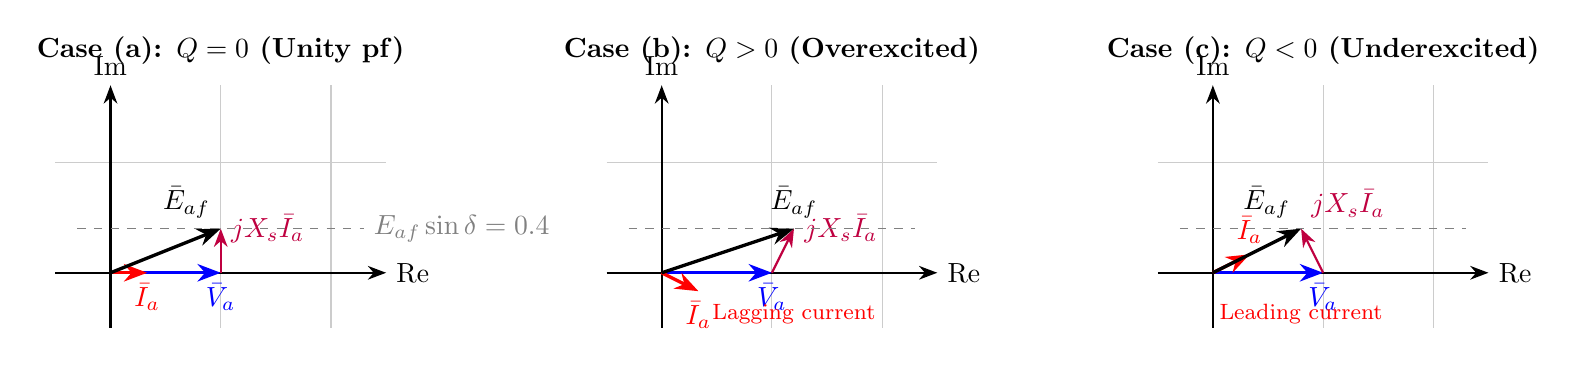
\begin{tikzpicture}[scale=1.4, >=Stealth]
        % Case (a): Unity
        \begin{scope}[xshift=0cm]
            \node[above, font=\bfseries] at (1, 1.8) {Case (a): $Q = 0$ (Unity pf)};
            \draw[thin, gray!40] (-0.5,-0.5) grid (2.5,1.7);
            \draw[->, thick] (-0.5,0) -- (2.5,0) node[right] {$\text{Re}$};
            \draw[->, thick] (0,-0.5) -- (0,1.7) node[above] {$\text{Im}$};
            
            % Va
            \draw[->, very thick, blue] (0,0) -- (1,0) node[below] {$\bar{V}_a$};
            % Ia
            \draw[->, very thick, red] (0,0) -- (0.333,0) node[below] {$\bar{I}_a$};
            % jXs Ia
            \draw[->, thick, purple] (1,0) -- (1,0.4) node[right] {$j X_s \bar{I}_a$};
            % Eaf
            \draw[->, very thick, black] (0,0) -- (1,0.4) node[above left] {$\bar{E}_{af}$};
            \draw[dashed, gray] (-0.3,0.4) -- (2.3,0.4) node[right] {$E_{af}\sin\delta = 0.4$};
        \end{scope}

        % Case (b): Overexcited
        \begin{scope}[xshift=5cm]
            \node[above, font=\bfseries] at (1, 1.8) {Case (b): $Q > 0$ (Overexcited)};
            \draw[thin, gray!40] (-0.5,-0.5) grid (2.5,1.7);
            \draw[->, thick] (-0.5,0) -- (2.5,0) node[right] {$\text{Re}$};
            \draw[->, thick] (0,-0.5) -- (0,1.7) node[above] {$\text{Im}$};
            
            % Va
            \draw[->, very thick, blue] (0,0) -- (1,0) node[below] {$\bar{V}_a$};
            % Ia
            \draw[->, very thick, red] (0,0) -- (0.333,-0.167) node[below] {$\bar{I}_a$};
            % jXs Ia
            \draw[->, thick, purple] (1,0) -- (1.2,0.4) node[right] {$j X_s \bar{I}_a$};
            % Eaf
            \draw[->, very thick, black] (0,0) -- (1.2,0.4) node[above] {$\bar{E}_{af}$};
            \draw[dashed, gray] (-0.3,0.4) -- (2.3,0.4);
            \node[below, red, font=\footnotesize] at (1.2,-0.2) {Lagging current};
        \end{scope}

        % Case (c): Underexcited
        \begin{scope}[xshift=10cm]
            \node[above, font=\bfseries] at (1, 1.8) {Case (c): $Q < 0$ (Underexcited)};
            \draw[thin, gray!40] (-0.5,-0.5) grid (2.5,1.7);
            \draw[->, thick] (-0.5,0) -- (2.5,0) node[right] {$\text{Re}$};
            \draw[->, thick] (0,-0.5) -- (0,1.7) node[above] {$\text{Im}$};
            
            % Va
            \draw[->, very thick, blue] (0,0) -- (1,0) node[below] {$\bar{V}_a$};
            % Ia
            \draw[->, very thick, red] (0,0) -- (0.333,0.167) node[above] {$\bar{I}_a$};
            % jXs Ia
            \draw[->, thick, purple] (1,0) -- (0.8,0.4) node[above right] {$j X_s \bar{I}_a$};
            % Eaf
            \draw[->, very thick, black] (0,0) -- (0.8,0.4) node[above left] {$\bar{E}_{af}$};
            \draw[dashed, gray] (-0.3,0.4) -- (2.3,0.4);
            \node[below, red, font=\footnotesize] at (0.8,-0.2) {Leading current};
        \end{scope}
    \end{tikzpicture}
    }
    \caption{Phasor diagrams of synchronous generator operating at constant active power $P$ under variable excitation.}
    \label{fig:tp5_phasors}
\end{figure}

\paragraph{Physical Explanation of Generator Voltage Control:}
\begin{itemize}
    \item \textbf{Overexcitation (Case b):}
    By increasing the rotor field current $I_f$, the internal EMF magnitude $|E_{af}|$ increases. Because $P$ is held constant, $\delta$ must decrease while $\bar{I}_a$ shifts into the lagging quadrant. The generator delivers reactive power to the grid ($Q > 0$), effectively acting as a \textbf{shunt capacitor}.
    
    \item \textbf{Underexcitation (Case c):}
    By decreasing the field current $I_f$, $|E_{af}|$ decreases. The current shifts into the leading quadrant, and the generator absorbs reactive power from the grid ($Q < 0$), acting as a \textbf{shunt inductor}.
    
    This capability to continuously adjust reactive power by varying the field current forms the foundation of \textbf{Automatic Voltage Regulation (AVR)} in bulk power transmission networks.
\end{itemize}

\subsubsection*{Solution to Exercise 3: Subtransient, Transient, and Steady-State Regimes}
\paragraph{Data:}
\begin{itemize}
    \item Armature resistance: $R_s = 0$
    \item Steady-state synchronous reactance: $X_s = 1.2\ \text{pu}$
    \item Transient reactance: $X_s' = 0.33\ \text{pu}$
    \item Subtransient reactance: $X_s'' = 0.23\ \text{pu}$
    \item Terminal voltage: $\bar{V}_a = 1\angle 0^\circ\ \text{pu}$
    \item Current: $\bar{I}_a = 1\angle -\pi/6\ \text{pu} = 1\angle -30^\circ\ \text{pu} = (0.866 - j0.5)\ \text{pu}$
\end{itemize}

\paragraph{1. Internal Voltages in each Regime:}
Using $\bar{E} = \bar{V}_a + j X \bar{I}_a$:
\begin{enumerate}[(a)]
    \item \textbf{Steady-State Voltage $\bar{E}_{af}$:}
    \begin{align}
        \bar{E}_{af} &= 1 + j 1.2(0.866 - j0.5) = 1 + 0.6 + j 1.0392 = 1.6 + j 1.0392\ \text{pu} \nonumber\\
                     &= \boxed{\mathbf{1.908\ \text{pu} \angle 33.0^\circ \quad (0.58\ \text{rad})}}
    \end{align}

    \item \textbf{Transient Voltage $\bar{E}_{af}'$:}
    \begin{align}
        \bar{E}_{af}' &= 1 + j 0.33(0.866 - j0.5) = 1 + 0.165 + j 0.2858 = 1.165 + j 0.2858\ \text{pu} \nonumber\\
                      &= \boxed{\mathbf{1.200\ \text{pu} \angle 13.78^\circ \quad (0.24\ \text{rad})}}
    \end{align}

    \item \textbf{Subtransient Voltage $\bar{E}_{af}''$:}
    \begin{align}
        \bar{E}_{af}'' &= 1 + j 0.23(0.866 - j0.5) = 1 + 0.115 + j 0.1992 = 1.115 + j 0.1992\ \text{pu} \nonumber\\
                       &= \boxed{\mathbf{1.133\ \text{pu} \angle 10.13^\circ \quad (0.18\ \text{rad})}}
    \end{align}
\end{enumerate}

\paragraph{2. Comparison and Physical Interpretation:}
\begin{equation}
    X_s'' < X_s' < X_s \iff 0.23 < 0.33 < 1.20\ \text{pu}
\end{equation}
\begin{equation}
    |E_{af}''| < |E_{af}'| < |E_{af}| \iff 1.13 < 1.20 < 1.91\ \text{pu}
\end{equation}
\begin{equation}
    \delta'' < \delta' < \delta \iff 10.1^\circ < 13.8^\circ < 33.0^\circ
\end{equation}

\paragraph{Physical Mechanism of the Three Time Frames:}
\begin{itemize}
    \item \textbf{Subtransient Period ($t \approx 10 - 20\ \text{ms}$, first few cycles):}
    When a sudden electrical fault or disturbance occurs, flux linkages in both the \textbf{damper windings} (amortisseur) and the rotor field winding cannot change instantaneously (Lenz's law). Heavy eddy currents are induced in the damper bars, trapping the flux in high-reluctance leakage paths outside the rotor body. Consequently, the equivalent reactance $X_s''$ is minimal, and the initial fault current is very large.
    
    \item \textbf{Transient Period ($t \approx 0.1 - 1.0\ \text{s}$):}
    Due to the high resistance of the damper bars, the subtransient damper currents rapidly decay with time constant $T_d''$. Flux is now prevented from changing only by the main field winding, whose resistance is much smaller. The corresponding effective reactance is $X_s'$, and the internal voltage is $\bar{E}_{af}'$.
    
    \item \textbf{Steady-State Period ($t > 1 - 2\ \text{s}$):}
    After several seconds, all induced transient rotor currents have fully dissipated. The field winding carries only DC excitation current supplied by the exciter, and the effective reactance increases to its full steady-state value $X_s$ (governed by stator leakage plus the full armature reaction mmf).
\end{itemize}

\newpage

\section{Practical Session 6: Voltage Instability in Power Systems}

\subsection{Exercises}
\begin{enumerate}
    \item \textbf{Derivation of the $P$-$V$ Characteristic of a Transmission Line}\footnote{Exercise from Practical Session 6: Voltage instability in power systems.}
    
    Consider the transmission system represented in Figure~\ref{fig:tp6_system}. A load consuming an active power $P$ and a reactive power $Q$ is connected to bus~2. The voltage phasor at bus~2 is:
    \[
    \bar{V} = V\angle\delta.
    \]
    A synchronous generator is connected to bus~1 and regulates the voltage at that bus to:
    \[
    \bar{E} = E\angle 0^\circ.
    \]
    The transmission line between bus~1 and bus~2 is assumed to be lossless with series reactance $X$, and the reactive power limits of the generator are not considered.

    \begin{figure}[htbp]
        \centering
        \begin{circuitikz}[american, scale=1.1]
            % Generator at bus 1
            \draw (0,0) to[sV, v_>=$\bar{E}$] (0,2)
                  -- (1.5,2) coordinate (bus1_top);
            \draw (0,0) -- (1.5,0) coordinate (bus1_bot);

            % Bus 1 bar
            \draw[ultra thick] (1.5,-0.5) -- (1.5,2.5);
            \node[below=0.6cm] at (1.5,0) {$\text{bus } 1$};
            \node[above] at (1.5,2.5) {$\bar{E} = E\angle 0^\circ$};

            % Line reactance jX
            \draw (1.5,1.5) to[L, l=$jX$, i=$\bar{I}$] (5.5,1.5) coordinate (bus2_in);

            % Bus 2 bar
            \draw[ultra thick] (5.5,-0.5) -- (5.5,2.5);
            \node[below=0.6cm] at (5.5,0) {$\text{bus } 2$};
            \node[above] at (5.5,2.5) {$\bar{V} = V\angle\delta$};

            % Load at bus 2
            \draw[->, very thick] (5.5,1.0) -- (6.8,1.0) -- (6.8,-0.2) node[below] {$S = P + jQ$};
            \draw[dashed, gray] (1.5,0) -- (5.5,0);
        \end{circuitikz}
        \caption{Single-line representation of a lossless transmission line feeding a load.}
        \label{fig:tp6_system}
    \end{figure}

    Based on these assumptions:
    \begin{enumerate}
        \item Derive the mathematical relationship between the active power $P$ consumed by the load and the receiving-end voltage magnitude $V$ at bus~2, for a constant load power factor angle $\phi$ ($Q = P\tan\phi$).
        \item Derive the mathematical expression of the maximum active power $P_{\text{max}}$ transmissible through the line.
        \item Identify and discuss the critical parameters to consider in order to transmit more power through the line.
    \end{enumerate}
\end{enumerate}

\newpage
\subsection{Solutions}

\subsubsection*{1. Derivation of the Relationship Between Load Active Power $P$ and Voltage Magnitude $V$}

\paragraph{Complex Power Flow Equations:}
The complex power $S$ consumed by the load at bus~2 is:
\begin{equation}
    S = P + jQ = \bar{V} \bar{I}^*
\end{equation}
The line current flowing from bus~1 to bus~2 through the reactance $jX$ is:
\begin{equation}
    \bar{I} = \frac{\bar{E} - \bar{V}}{jX}
\end{equation}
Substituting this current into the complex power expression:
\begin{align}
    S &= \bar{V} \left( \frac{\bar{E} - \bar{V}}{jX} \right)^* = (V\angle\delta) \left( \frac{E - V\angle\delta}{jX} \right)^*
\end{align}
Using the complex conjugate identity $\left(\frac{1}{j}\right)^* = (-j)^* = j$:
\begin{align}
    S &= V\angle\delta \left( -j \frac{E - V\angle\delta}{X} \right)^* = V\angle\delta \left( j \frac{E - V\angle(-\delta)}{X} \right) \nonumber\\
      &= \frac{V}{X} \angle\delta \left[ j E - j V(\cos\delta - j\sin\delta) \right] \nonumber\\
      &= \frac{V}{X} \angle\delta \left[ -V\sin\delta + j(E - V\cos\delta) \right] \nonumber\\
      &= \frac{V}{X} (\cos\delta + j\sin\delta) \left[ -V\sin\delta + j(E - V\cos\delta) \right]
\end{align}

Expanding the product into real and imaginary parts:
\paragraph{Active Power $P$:}
\begin{align}
    P = \text{Re}\{S\} &= \frac{V}{X} \left[ \cos\delta (-V\sin\delta) + \sin\delta (E - V\cos\delta) \right] \nonumber\\
                       &= \frac{V}{X} \left[ -V\cos\delta\sin\delta + E\sin\delta - V\sin\delta\cos\delta \right] \nonumber\\
                       &= \boxed{\frac{EV}{X} \sin(-\delta) = -\frac{EV}{X}\sin\delta} \label{eq:tp6_P}
\end{align}
Taking the convention where $\delta < 0$ (load voltage lags the source voltage), let $\theta = -\delta > 0$:
\begin{equation}
    P = \frac{EV}{X} \sin\theta
\end{equation}

\paragraph{Reactive Power $Q$:}
\begin{align}
    Q = \text{Im}\{S\} &= \frac{V}{X} \left[ \cos\delta (E - V\cos\delta) - \sin\delta (-V\sin\delta) \right] \nonumber\\
                       &= \frac{V}{X} \left[ E\cos\delta - V\cos^2\delta + V\sin^2\delta \right] \nonumber\\
                       &= \boxed{\frac{V}{X} (E\cos\delta - V)} \label{eq:tp6_Q}
\end{align}

\paragraph{Eliminating the Phase Angle $\delta$:}
From equations~\eqref{eq:tp6_P} and~\eqref{eq:tp6_Q}:
\begin{align}
    \sin\delta &= -\frac{PX}{EV} \label{eq:tp6_sindelta}\\
    \cos\delta &= \frac{QX + V^2}{EV} \label{eq:tp6_cosdelta}
\end{align}
Applying the trigonometric identity $\sin^2\delta + \cos^2\delta = 1$:
\begin{equation}
    \left( \frac{PX}{EV} \right)^2 + \left( \frac{QX + V^2}{EV} \right)^2 = 1
\end{equation}
Multiplying through by $(EV)^2$:
\begin{equation}
    P^2 X^2 + (QX + V^2)^2 = E^2 V^2
\end{equation}
Expanding the second term:
\begin{equation}
    P^2 X^2 + Q^2 X^2 + 2 Q X V^2 + V^4 = E^2 V^2
\end{equation}
Grouping terms into a quadratic polynomial in $V^2$:
\begin{equation}
    \boxed{V^4 + (2QX - E^2) V^2 + X^2(P^2 + Q^2) = 0} \label{eq:tp6_biquadratic}
\end{equation}

\paragraph{Solving for the Voltage Magnitude $V$:}
Let $y = V^2$. The quadratic equation is $y^2 + (2QX - E^2)y + X^2(P^2 + Q^2) = 0$.
Applying the quadratic formula:
\begin{align}
    y &= \frac{-(2QX - E^2) \pm \sqrt{(2QX - E^2)^2 - 4 X^2 (P^2 + Q^2)}}{2} \nonumber\\
      &= \frac{E^2 - 2QX \pm \sqrt{4Q^2 X^2 - 4 E^2 Q X + E^4 - 4 P^2 X^2 - 4 Q^2 X^2}}{2} \nonumber\\
      &= \frac{E^2}{2} - QX \pm \sqrt{\frac{E^4}{4} - E^2 Q X - P^2 X^2}
\end{align}
Taking the square root to obtain the voltage magnitude $V = \sqrt{y}$:
\begin{equation}
    \boxed{V = \sqrt{\frac{E^2}{2} - QX \pm \sqrt{\frac{E^4}{4} - E^2 Q X - P^2 X^2}}} \label{eq:tp6_V_sol}
\end{equation}
For a load operating at a constant power factor $\cos\phi$, the reactive power is proportional to active power:
\begin{equation}
    Q = P \tan\phi
\end{equation}
where $\phi > 0$ for inductive (lagging) loads and $\phi < 0$ for capacitive (leading) loads.
Substituting $Q = P\tan\phi$ into~\eqref{eq:tp6_V_sol}:
\begin{equation}
    \boxed{V = \sqrt{\frac{E^2}{2} - X(P\tan\phi) \pm \sqrt{\frac{E^4}{4} - E^2 X (P\tan\phi) - X^2 P^2}}}
\end{equation}
This equation describes the classical \textbf{$P$-$V$ nose curve} of the transmission line.
For each valid power $P < P_{\text{max}}$, there are two mathematical voltage solutions:
\begin{itemize}
    \item \textbf{Upper branch ($+$ sign):} High voltage, low current, physically stable operating point.
    \item \textbf{Lower branch ($-$ sign):} Low voltage, high current, unstable operating point.
\end{itemize}

\subsubsection*{2. Maximum Transmissible Active Power $P_{\text{max}}$}
The maximum transmissible power $P_{\text{max}}$ occurs at the \textbf{nose} (turning point / saddle-node bifurcation) of the $P$-$V$ curve, where the two voltage solutions merge into a single unique point.
This condition is reached when the discriminant $\Delta$ under the inner square root vanishes:
\begin{equation}
    \Delta = \frac{E^4}{4} - E^2 X (P_{\text{max}}\tan\phi) - X^2 P_{\text{max}}^2 = 0
\end{equation}
Rearranging into standard quadratic form for $P_{\text{max}}$:
\begin{equation}
    X^2 P_{\text{max}}^2 + (E^2 X \tan\phi) P_{\text{max}} - \frac{E^4}{4} = 0
\end{equation}
Dividing by $X^2$:
\begin{equation}
    P_{\text{max}}^2 + \left(\frac{E^2 \tan\phi}{X}\right) P_{\text{max}} - \frac{E^4}{4 X^2} = 0
\end{equation}
Using the quadratic formula and selecting the positive physical root:
\begin{align}
    P_{\text{max}} &= \frac{-\left(\frac{E^2\tan\phi}{X}\right) + \sqrt{\left(\frac{E^2\tan\phi}{X}\right)^2 - 4(1)\left(-\frac{E^4}{4X^2}\right)}}{2} \nonumber\\
                   &= \frac{1}{2} \left[ -\frac{E^2\tan\phi}{X} + \sqrt{\frac{E^4\tan^2\phi}{X^2} + \frac{E^4}{X^2}} \right] \nonumber\\
                   &= \frac{E^2}{2X} \left[ -\tan\phi + \sqrt{\tan^2\phi + 1} \right]
\end{align}
Using the trigonometric identity $1 + \tan^2\phi = \sec^2\phi = \frac{1}{\cos^2\phi}$:
\begin{equation}
    \sqrt{1 + \tan^2\phi} = \frac{1}{\cos\phi}
\end{equation}
Substituting $\tan\phi = \frac{\sin\phi}{\cos\phi}$:
\begin{align}
    P_{\text{max}} &= \frac{E^2}{2X} \left[ -\frac{\sin\phi}{\cos\phi} + \frac{1}{\cos\phi} \right] \nonumber\\
                   &= \boxed{\frac{E^2}{2X} \left( \frac{1 - \sin\phi}{\cos\phi} \right)} \label{eq:tp6_Pmax}
\end{align}

\paragraph{Critical Voltage at the Limit:}
At $P = P_{\text{max}}$, the inner discriminant is zero, so:
\begin{equation}
    V_{\text{crit}} = \sqrt{\frac{E^2}{2} - X Q_{\text{crit}}} = \sqrt{\frac{E^2}{2} - X P_{\text{max}}\tan\phi}
\end{equation}
Substituting $P_{\text{max}}$ from~\eqref{eq:tp6_Pmax}:
\begin{align}
    V_{\text{crit}}^2 &= \frac{E^2}{2} - X \left[\frac{E^2}{2X}\left(\frac{1 - \sin\phi}{\cos\phi}\right)\right] \frac{\sin\phi}{\cos\phi} \nonumber\\
                     &= \frac{E^2}{2} \left[ 1 - \frac{\sin\phi - \sin^2\phi}{\cos^2\phi} \right] = \frac{E^2}{2} \left[ \frac{\cos^2\phi - \sin\phi + \sin^2\phi}{\cos^2\phi} \right] \nonumber\\
                     &= \frac{E^2}{2} \left[ \frac{1 - \sin\phi}{1 - \sin^2\phi} \right] = \frac{E^2}{2(1 + \sin\phi)}
\end{align}
\begin{equation}
    \boxed{V_{\text{crit}} = \frac{E}{\sqrt{2(1 + \sin\phi)}}}
\end{equation}
For a purely resistive load ($\phi = 0$):
\[
P_{\text{max}} = \frac{E^2}{2X}, \quad V_{\text{crit}} = \frac{E}{\sqrt{2}} \approx 0.707 E
\]

\subsubsection*{3. Key Parameters Influencing the Maximum Transmissible Power}
From equation~\eqref{eq:tp6_Pmax}, three primary parameters determine the transmission limit:
\begin{enumerate}
    \item \textbf{Sending-End Voltage Magnitude ($E$):}
    The maximum power increases quadratically with the sending-end voltage:
    \[
    P_{\text{max}} \propto E^2
    \]
    Operating transmission grids at higher voltage levels (e.g., $400\ \text{kV}$ or $765\ \text{kV}$) drastically increases the capacity of corridors.

    \item \textbf{Line Series Reactance ($X$):}
    The maximum transmissible power is inversely proportional to the line reactance:
    \[
    P_{\text{max}} \propto \frac{1}{X}
    \]
    To increase capacity on an existing corridor:
    \begin{itemize}
        \item Install \textbf{series capacitor banks} (series compensation) to reduce net line reactance: $X_{\text{eff}} = X_{\text{line}} - X_C$.
        \item Construct parallel circuits or bundle multiple sub-conductors per phase to decrease line inductance.
    \end{itemize}

    \item \textbf{Load Power Factor ($\cos\phi$ and Angle $\phi$):}
    The factor $\frac{1 - \sin\phi}{\cos\phi}$ depends strongly on the power factor:
    \begin{itemize}
        \item \textbf{Inductive loads ($\phi > 0$, lagging pf):} $\sin\phi > 0 \implies \frac{1 - \sin\phi}{\cos\phi} < 1$, reducing $P_{\text{max}}$ significantly and worsening voltage drop.
        \item \textbf{Capacitive loads ($\phi < 0$, leading pf):} $\sin\phi < 0 \implies \frac{1 - \sin\phi}{\cos\phi} > 1$, raising the maximum power limit and supporting voltage.
    \end{itemize}
    This underscores why shunt capacitors, STATCOMs, and SVCs are installed near load centers: by providing local reactive power support, they unload the line from transmitting reactive power, effectively increasing the active power transfer capability and preventing voltage collapse.
\end{enumerate}


\end{document}
